\chapter{Extension aux surfaces courbes}
\label{chap:surface_courbe}
\minitoc

\[\]

Dans ce chapitre, nous exposons une généralisation des notions abordés au deux chapitres précédents au cas des surfaces courbes dans l'espace. Plus précisement, on considère $\Omega$ comme une surface compacte orienté plongé dans $\mathbb{R}^3$. Pour tout point $p\in\Omega$ nous notons $N(p)$ la normale à la surface (autrement dit le vecteur normale à l'espace tangent $T_p\Omega$).

\section{Champ de croix, points singuliers, indices et séparatrices}

Dans cette section, nous revisitions les définitions et concepts introduits dans le chapitre \ref{chap:theoritical}. Un champ de croix $\bar{u}$ défini sur $\Omega$ associe à chaque point $p$ de $\Omega$ une croix (voir la définition \ref{def:croix}) définie dans l'espace tangent $T_p\Omega$. L'ensemble $\mathcal{S}_{\bar{u}_h}$, désignant l'ensemble des points singuliers de $\bar{u}_h$, est formé des points $p \in \Omega_h$ tels que $\bar{u}_h(p) = 0$ et on dira que le champ de croix est presque-$\mathcal{C}^1$ s'il satisfait à la définition \ref{def:presqueC1}. En ajustant l'opérateur de rotation de manière à ce que la rotation d'une croix s'effectue autour de la normale surfacique définie au point, la proposition \ref{prop:cont1} permet de réaliser la rotation d'un champ de croix défini sur une surface par rapport à un champ d'angle défini sur cette même surface.

Contrairement au cas planaire où l'on disposais d'une réference globale pour le calcul des angles des croix, ici on se donne une référence arbitraire en chaque espace tangent de la surface permettant ainsi de calculer l'angle de la croix relativement à cette référence. On retrouve alors la formule de l'indice d'un point $p$ dans un champ de croix presque-$\mathcal{C}^1$ défini sur $\Omega$:

\begin{equation}
\label{eqn:index_surf}
    id_{\bar{u}}(p)=\displaystyle\frac{1}{2\pi}\int_0^1 d\theta_{\bar{u}}^\gamma.
\end{equation}
La définition des lignes de champ des champs de croix sur les surfaces courbes ainsi que les propriétés des séparatrices demeurent valident dans ce nouveau cadre. Cependant, notons que pour l'intégration des lignes de champ à partir de points singuliers (séparatrices), le voisinnage étoilé permettant de modifier localement le champde croix pour permettre le démarragede la séparatrices doit être de taille assez petit. Plus concrètement, il faut que ce voisinnage soit homémorphe au plan pour pouvoir mettre en oeuvre l'opération de modification du champ que nous avons introduit dans la proposition \ref{prop:stream_from_interior_sing}. A partir de là, on retrouve facilement les résultat concernant le lien entre le nombre de séparatrice associé à un point singulier et l'indice du point.

Examinons maintenant ce que devient ces concepts dans un cadre discret. Soit $\Omega_h$ un maillage triangulaire de $\Omega$ vérifiant les contraintes définis dans la sous-section \ref{subsec:mesh_tri} et soit $\bar{u}$ un champ de croix presque-$\mathcal{C}^1$ défini sur $\Omega$.
\\
definition de delta avec cosinus\\
on definit ensuite les zone singuliere comme dans le chapitre 3\\
definir ensuite la represenatation en projetant sur les triangles\\


Nous cherchons maintenant à construire une représentation du champ de croix $\bar{u}$ sur le maillage triangulaire $\Omega_h$. Pour ce faire, nous allons nous orienter en nous basant sur les différentes opérations que nous devrons effectuer sur cette représentation en prenant comme modèle les opérations réalisées sur $\bar{u}$ dans le chapitre \ref{chap:theoritical}. Observons que nous devrons calculer la variation de l'angle des croix le long d'un arc paramétré, notamment pour déterminer l'indice de points ou pour quantifier la variation du champ de croix dans une partie du domaine. En limitant ces arcs aux bords des triangles, il devient évident qu'il est possible de simplifier le problème en connaissant la variation des croix le long des arêtes du triangle. En d'autres termes, il nous faut une notion de variation d'angle entre deux croix quelconques. Nous avons alors la définition suivante:

\begin{definition}
Soient deux croix $\mathbf{c}_1,\mathbf{c}_2$ non nulles. L'angle signé entre $\mathbf{c}_1$ et $\mathbf{c}_2$ noté $\delta\theta(\mathbf{c}_1,\mathbf{c}_2$) est l'unique élément de l'ensemble:
$$
\{\delta\theta(\mathbf{c}_1,\mathbf{c}_2)\}:=\left\{\theta_{\mathbf{c}_2}-\theta_{\mathbf{c}_1}+k\frac{\pi}{2},~k\in\mathbb{Z}\right\}\cap\left]-\frac{\pi}{4}, \frac{\pi}{4}\right[.
$$
\end{definition}
Cette fonction mesure la variation angulaire entre $\mathbf{c}_1$ et $\mathbf{c}_2$ de $\mathbf{c}_1$ vers $\mathbf{c}_2$. Autrement dit, on a:
$$
\theta_{\mathbf{c}_2}=\theta_{\mathbf{c}_1}+\delta\theta(\mathbf{c}_1,\mathbf{c}_2).
$$
Une conséquence directe de cette définition est l'antisymétrie de l'angle, ce qui se traduit par:
$$
\delta\theta(\mathbf{c}_1, \mathbf{c}_2)=-\delta\theta(\mathbf{c}_2,\mathbf{c}_1).
$$
Nous dirons que $\delta\theta(\mathbf{c}_1,\mathbf{c}_2$) n'est pas défini lorsque $|\theta_{\mathbf{c}_2}-\theta_{\mathbf{c}_1}|=\pi/4$.
Cette définition nous permet d'introduire l'assertion suivante.
\begin{assertion}
\label{ass:triangle_singulier}
 Soit triangle $T$ et de sommets $s_1$, $s_2$ et $s_3$ vérifiant l'une des propriétés suivantes:\\
 \begin{itemize}
  \item[1.] il existe $i\in\llbracket 1, 3\rrbracket$ tel que $\bar{u}(s_i)=0$,\\%[-0.2cm]
  \item[2.] il existe  $i,j\in\llbracket 1, 3\rrbracket$, tel que  $\delta\theta(\bar{u}(s_i),\bar{u}(s_{j}))$ n'est pas défini,\\%[-0.2cm]
  \item[3.] pour tout $i\in\llbracket 1, 3\rrbracket$, $\bar{u}(s_i)\neq 0$ et $\sum_{i=1}^3\delta\theta(\bar{u}(s_i),\bar{u}(s_{i+1}))\neq 0$ où on a posé $s_4:=s_1$.\\[-0.2cm]
 \end{itemize}
\end{assertion}

On peut subdiviser l'ensemble des triangles vérifiant l'assertion \ref{ass:triangle_singulier} en plusieurs partitions, dont les parties du plan correspondant seront appelées \emph{zones singulières}. Pour assembler ces partitions, on regroupe les triangles singuliers qui ont un ou plusieurs triangles singuliers comme voisins. Voici un exemple illustrant la construction de zones singulières sur la figure \ref{fig:zone_singuliere}. Dans ce cas, on se donne une configuration où la couleur rouge indique les lieux où l'une des propriétés de l'assertion \ref{ass:triangle_singulier} est vérifiée. Nous affichons ensuite les zones singulières correspondantes en bleu. Cette configuration particulière conduit à la création de cinq zones singulières que nous présentons sur la même figure. Dans la suite, nous utiliserons la notation $\mathbf{Z}=\cup_{i=1}^{N_Z}Z_i$ pour représenter la partie du plan occupé par l'ensemble des zones singulières. Ici, $Z_i$ désigne une zone singulière spécifique, et $N_z$ représente le nombre total de zones singulières. Ce nombre est nécessairefini puisque le champ de croix $\bar{u}$ possède un nombre fini de points singuliers. Nous associons ensuite à chaque zone singulière $Z\in \mathbf{Z}$ un point arbitrairement choisi dans $Z$, que nous notons $S_Z$ (par exemple, lorsque $Z$ est réduit à un unique triangle, on peut choisir $S_Z$ comme le barycentre du triangle en question).

\begin{figure}[h!]
\centering
\begin{subfigure}{0.49\textwidth}
    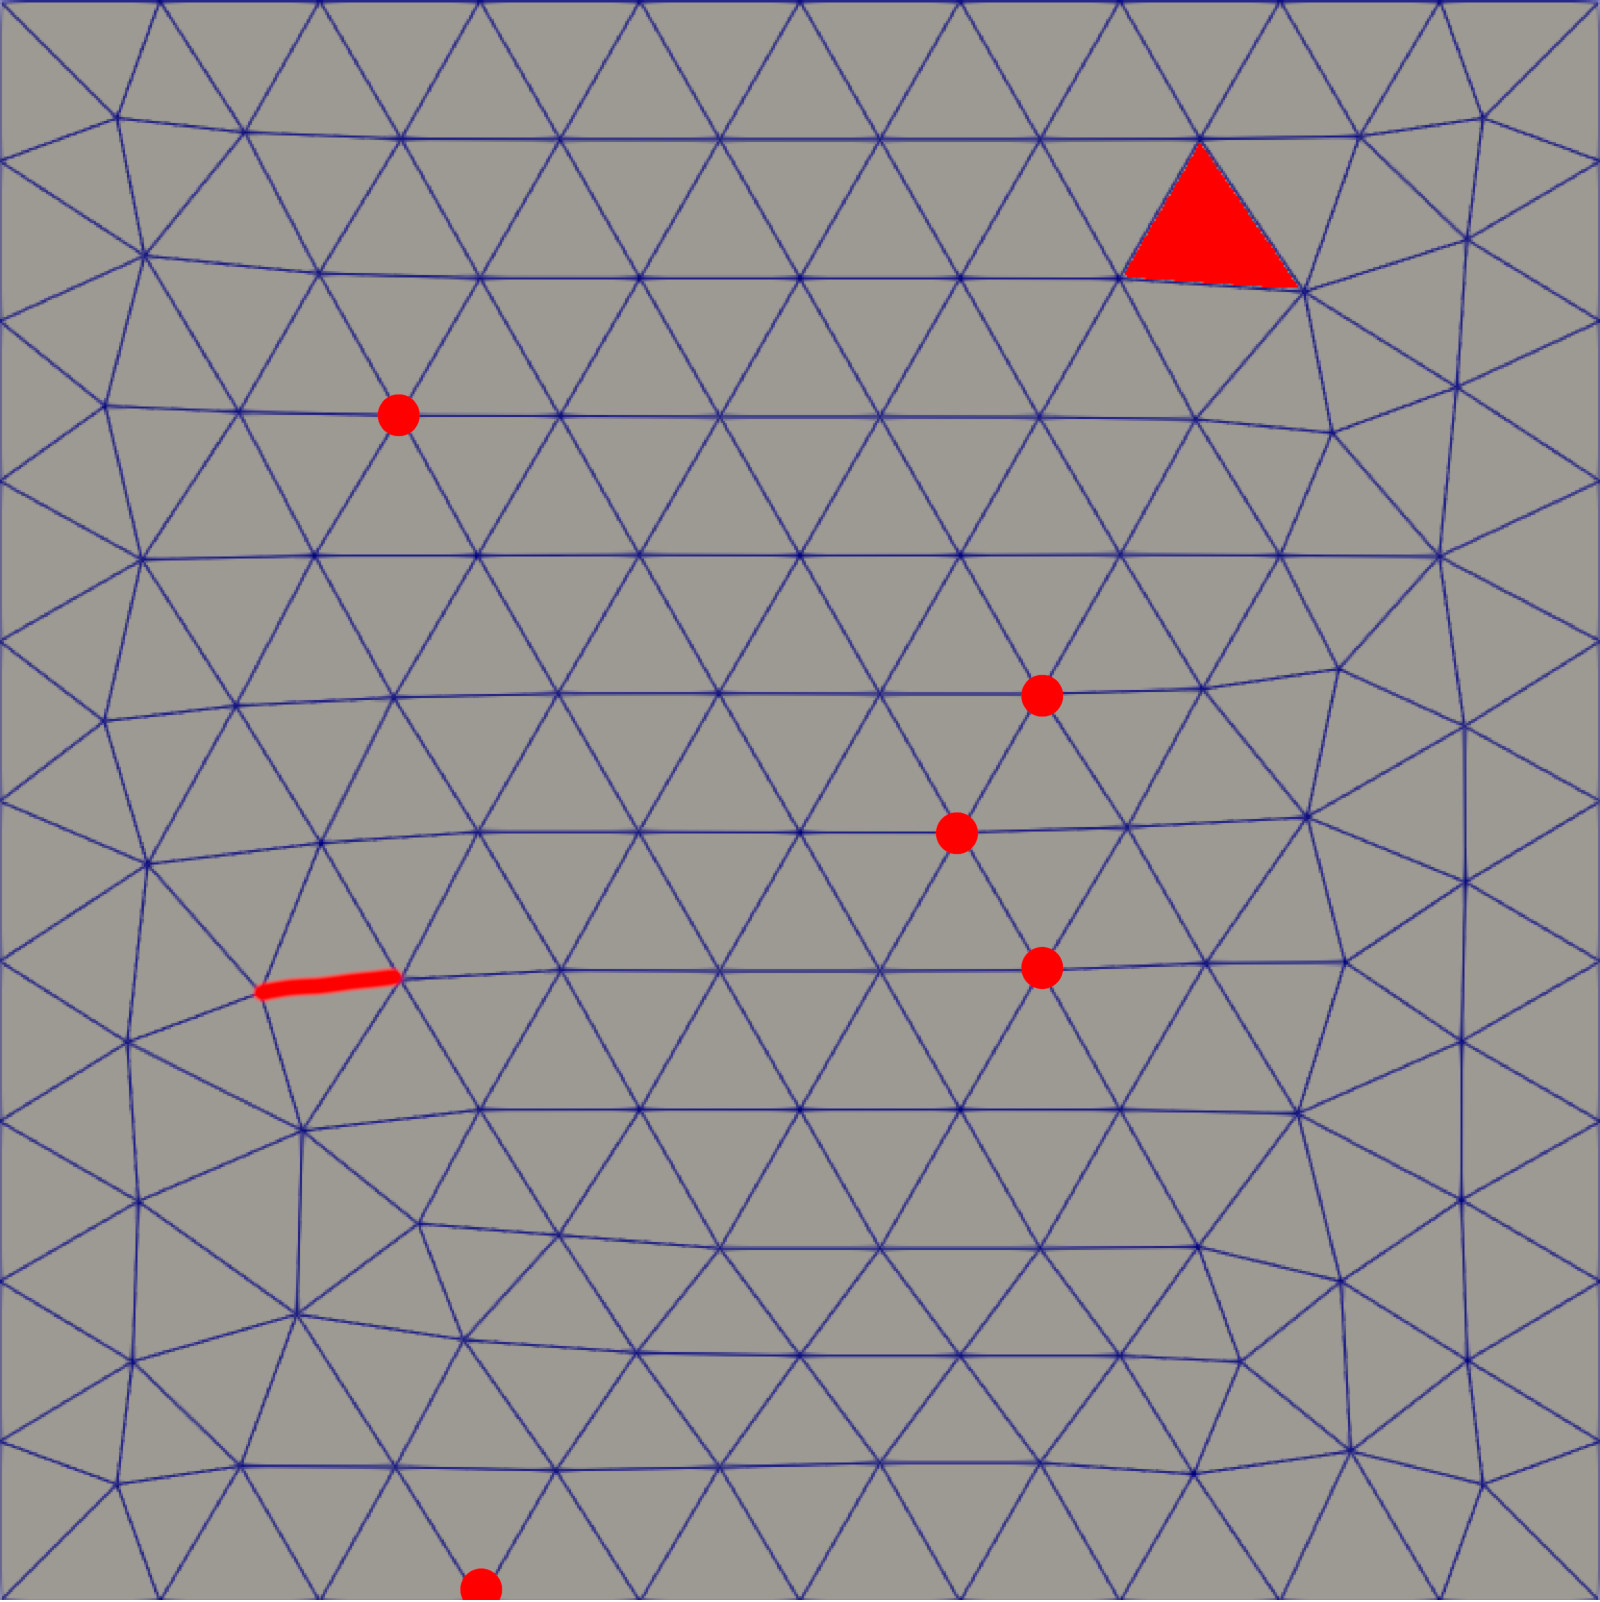
\includegraphics[width=\textwidth]{images/zone_singuliere_1.pdf}
    %\caption{Insertion de $D$.}
    %\label{fig:quad_eclatement}
\end{subfigure}
\hfill
\begin{subfigure}{0.49\textwidth}
    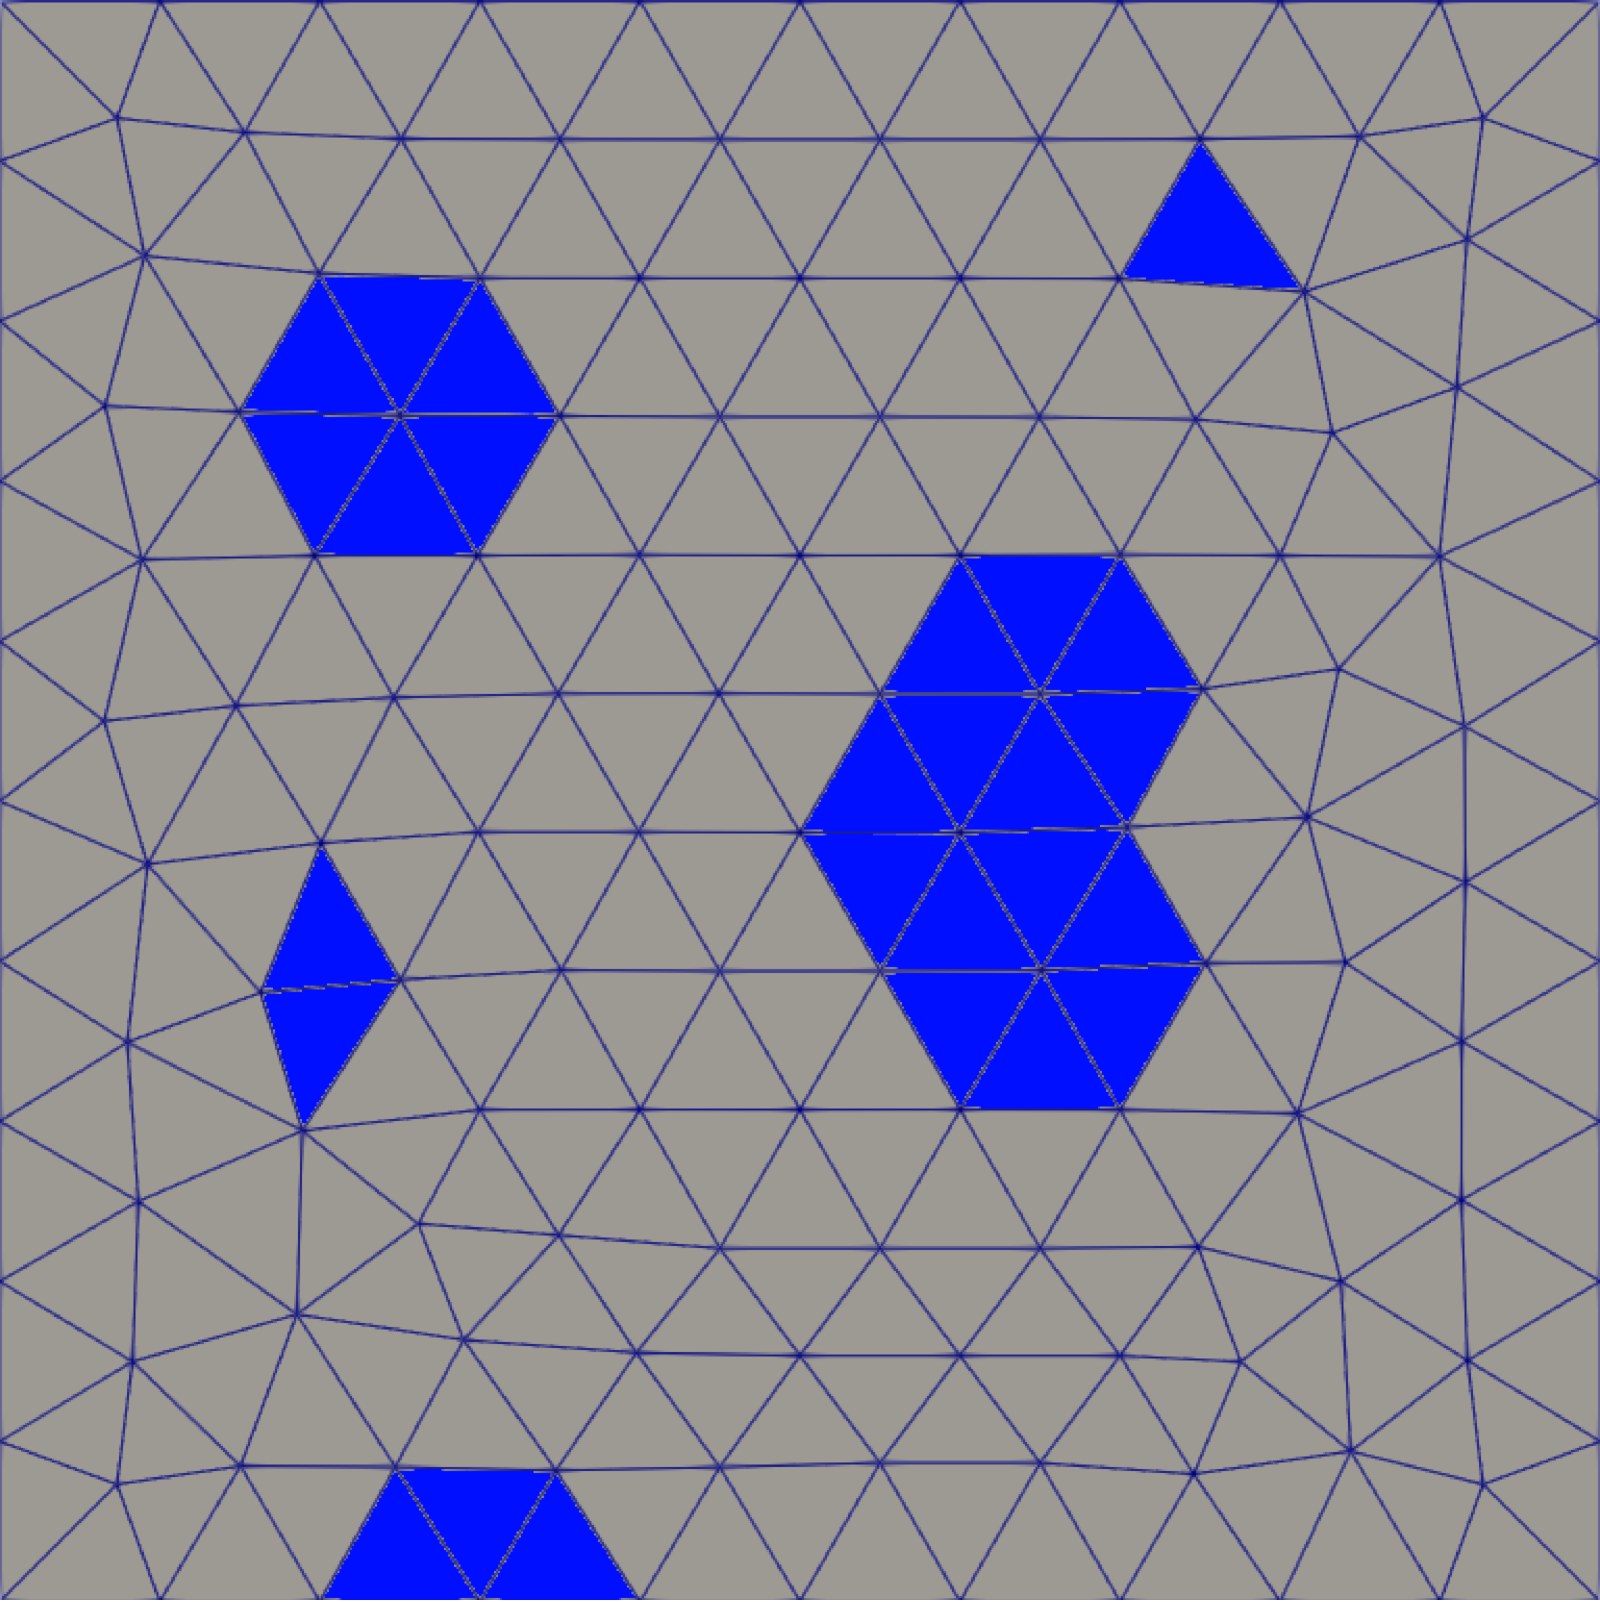
\includegraphics[width=\textwidth]{images/zone_singuliere_2.pdf}
    %\caption{Insertion de $E$.}
    %\label{fig:quad_carre}
\end{subfigure}
\caption{Illustration de la construction de zones singulières.}
\label{fig:zone_singuliere}
\end{figure}

Avec ces outils, nous sommes à présent en mesure de présenter notre proposition de représentation $\bar{u}_h$ sur $\Omega_h$ d'un champ de croix $\bar{u}$ défini sur $\Omega$. Pour tout $p\in\Omega_h$, nous définissons $\bar{u}_h$ de la manière suivante:\\

\begin{itemize}
\item[$\bullet$] si $p\in(\mathcal{S}_h\backslash\mathbf{Z})\cap\partial Z$, alors $\bar{u}_h(p)=\bar{u}(p)$.\\%[-0.3cm]
\item[$\bullet$] si $p\in\Omega_h\backslash\mathbf{Z}$ alors il existe $T\in\mathcal{T}_h$ tel que $p\in T$ et $T$ ne vérifie pas l'assertion \ref{ass:triangle_singulier}. On pose alors:
$$
\left\{
\begin{array}{l}
\theta_1 = \theta_{\bar{u}_h}(s_1)\\\\
\theta_2 = \theta_1 + \delta\theta(\bar{u}_h(s_1),\bar{u}_h(s_2))\\\\
\theta_3 = \theta_2 + \delta\theta(\bar{u}_h(s_2),\bar{u}_h(s_3))
\end{array}
\right.
$$
où $s_1$, $s_2$ et $s_3$ sont les sommets du triangle $T$. La croix $\bar{u}_h(p)$ est alors donnée par:
$$
\left\{
\begin{array}{l}
\bar{u}_h(p)=\displaystyle\left\{\mathbf{R}\left(\theta_p+m\frac{\pi}{2}\right)(1,0)^t,~m\in\mathbb{Z}\right\},\\\\
\theta_p=\displaystyle\sum_{i\in\llbracket1, 3\rrbracket}\lambda_i\theta_i,
\end{array}
\right.
$$
avec $(\lambda_i)_{i\in\llbracket 1, 3\rrbracket}$ les coordonnées barycentriques de $p$ dans le triangle $T$. Autrement dit, ils vérifient $p=\sum_{i=1}^3\lambda_i s_i$ et $\sum_{i=1}^3\lambda_i=1$.\\
\item[$\bullet$] si $p\in\mathbf{Z}$ alors il existe une zone singulière $Z\subset\mathbf{Z}$ tel que $p\in Z$. On a alors:\\
\begin{itemize}
 \item si $p=S_Z$, alors $\bar{u}_h(p)=0$.\\
 \item sinon la croix $\bar{u}_h(p)$ est donnée par:
\begin{equation}
\label{eqn:etoilage}
\left\{
\begin{array}{l}
\bar{u}_h(p)=\bar{u}_h(\widetilde{p}),\\\\
\{\widetilde{p}\}=[S_Zp)\cap\partial Z.
\end{array}
\right.
\end{equation}
Notons que l'ensemble $[S_Zp)\cap\partial Z$ est bien réduit à un singleton puisque $Z$ est une réunion de simplexes donc convexe.\\
\end{itemize}
\end{itemize}

\begin{remark}
La construction nous avons exposé se base sur l'angle signé entre les croix des arêtes du maillage. Plus précisément, nous utilisons les variations du champ de croix le long des arêtes pour construire notre représentation en chaque point et pour évaluer les indices des points singuliers. Ainsi, lorsque cette variation angulaire n'est pas définie, notre représentation induit des points singuliers non isolés, comme nous le verrons dans le lemme \ref{lem:isolation_pt_sing}.
Pour palier à ce désagrément, nous imposons dans toute la suite les conditions suivantes:\\
\begin{itemize}
 \item si on a $Z\subset\mathbf{Z}$ tel que $Z\cap\partial\Omega_h=\emptyset$, on doit avoir pour tout $p\in\partial Z\cap\mathcal{S}_h$, $\bar{u}(p)\neq 0$ et pour tout arête $s_1s_2\subset\partial Z$, $\delta\theta(\bar{u}(s_1),\bar{u}(s_2))$ doit être défini.\\
 \item si on a $Z\subset\mathbf{Z}$ tel que $Z\cap\partial\Omega_h\neq\emptyset$, on impose $S_Z\in\partial\Omega_h$ et on doit avoir pour tout $p\in(\partial Z\cap\mathcal{S}_h)\backslash\{S_Z\}$, $\bar{u}(p)\neq 0$ et pour tout arête $s_1s_2\subset\partial Z$, $\delta\theta(\bar{u}(s_1),\bar{u}(s_2))$ doit être défini.\\
\end{itemize}
Dans la pratique, il sera donc impératif de modifier un maillage qui ne satisfait pas ces contraintes. %La pertinence de ces contraintes prend tout son sens par la suite, avec l'approche de construction que nous proposons pour représenter $\bar{u}$ sur $\Omega_h$.
Étant donné que les points singuliers du champ de croix $\bar{u}$ sont isolés, on peut toujours satisfaire ces contraintes en affinant ou en modifiant localement (par exemple, par des opérations de retournement d'arêtes) un maillage qui ne satisfait pas ces contraintes.
\end{remark}



\begin{figure}[!h]
  \centering
  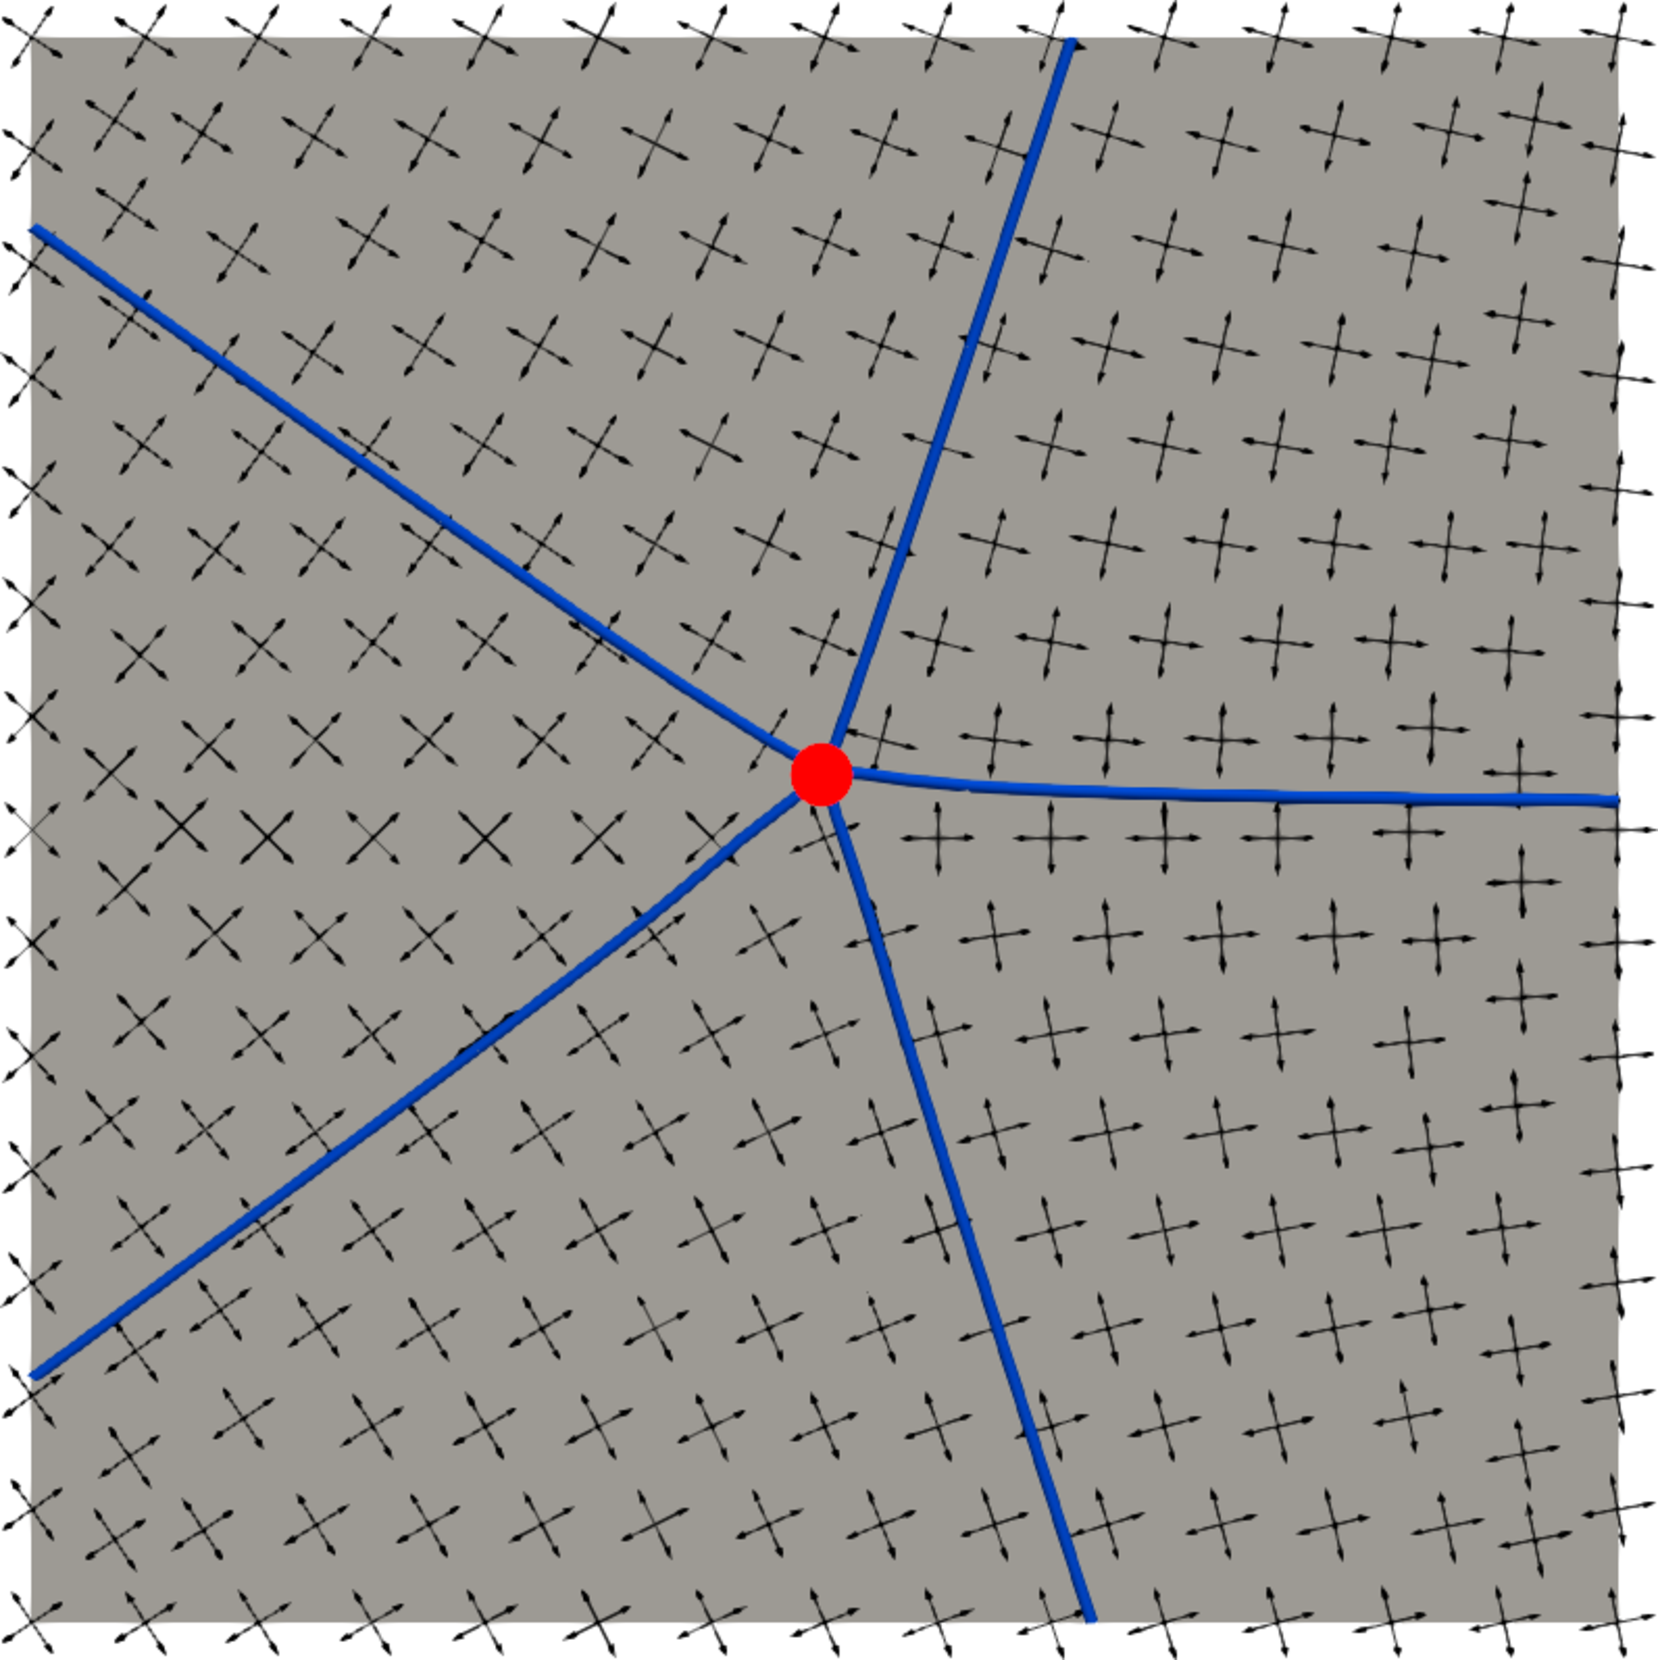
\includegraphics[scale=0.282]{images/sepa_5.pdf}
  \hfill
  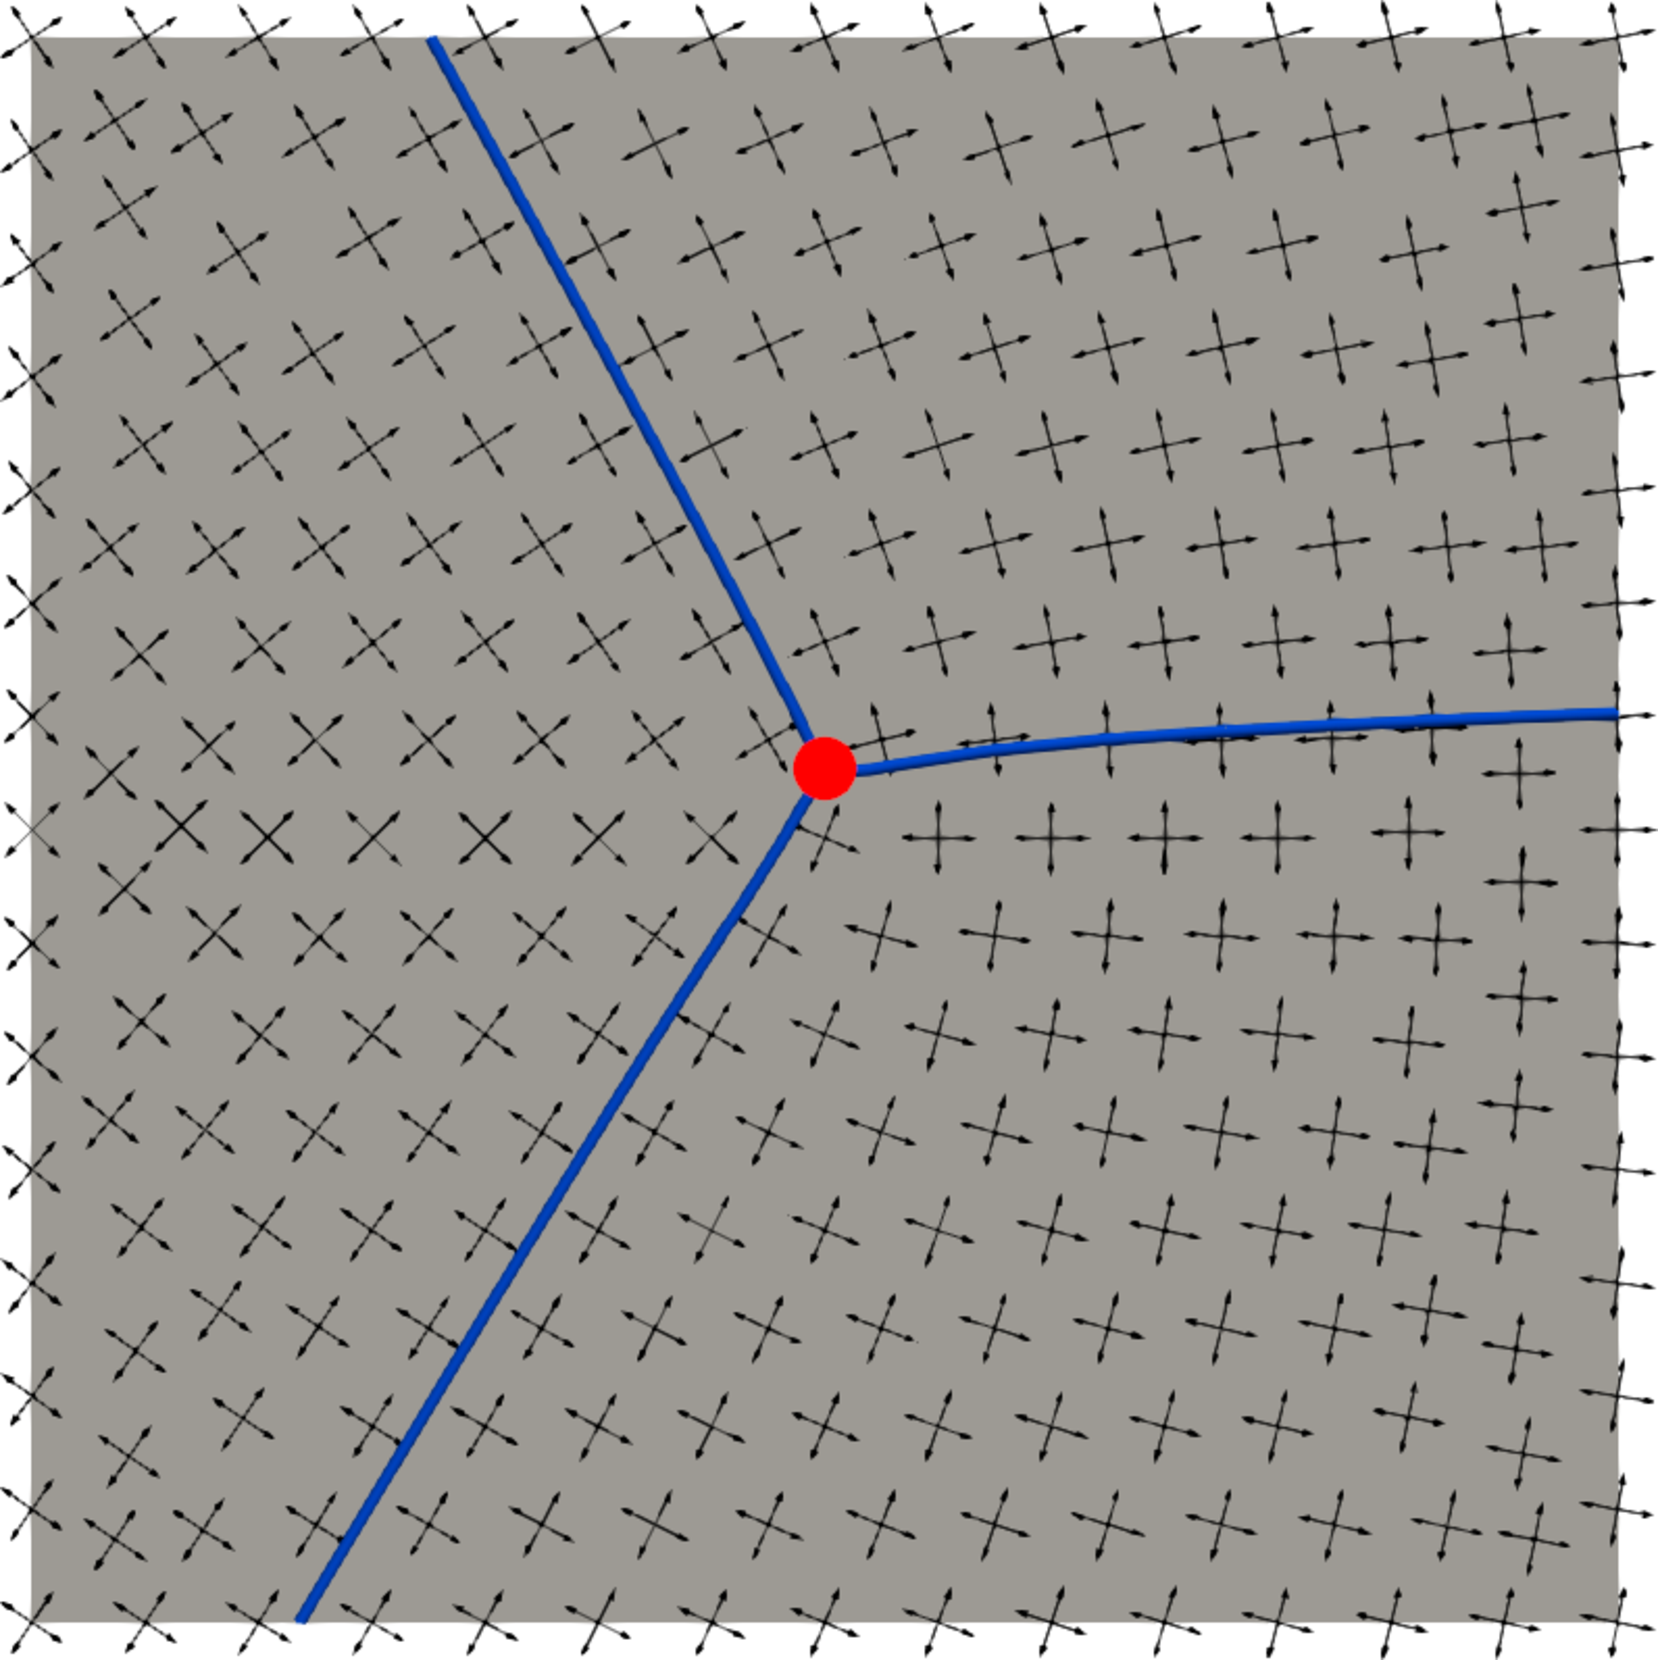
\includegraphics[scale=0.282]{images/sepa_3.pdf}
  \caption{Gauche: Illustration des séparatrices émanant de points singuliers d'indice $-1/4$ (à gauche) et d'indice $1/4$ (à droite).}
  \label{fig:separatrice_illustration}
\end{figure}

\begin{proposition}
\label{prop:loveprop}
Considérons un secteur tel que décrit ci-dessus. Lorsqu'il est traité comme une singularité de bord du secteur, le point $p$ a un indice de $1/4$.
\end{proposition}

\begin{proof}
Supposons que le secteur soit défini par deux séparatrices avec des directions initiales $\overrightarrow{p\gamma(t_i)}$ et $\overrightarrow{p\gamma(t_{i+1})}$, qui sont alignées avec la frontière du secteur. Soit $C$, la paramétrisation de la courbe définie par $p\gamma(t_i)$, $p\gamma(t_{i+1})$ et la partie de $\gamma$ coincé dans le secteur. L'indice de $p$ est alors donné par:
\begin{eqnarray*}
id^\partial_{\bar{u}}(p)&=&\frac{1}{2\pi}\left[\pi-\hat{p}+\lim\limits_{s\rightarrow 0}\int_{s-t_i}^{s-t_{i+1}}d\theta_{\bar{u}}^\gamma\right]\\
&=&\frac{1}{2\pi}\left[\pi-\hat{p}+\left(\hat{p}+\lim\limits_{s\rightarrow 0}\int_{s-t_i}^{s-t_{i+1}}dW_p^\gamma\right)\right]\\
&=&\frac{1}{2\pi}\left[\pi-\frac{\pi}{2}\right]\\
id^\partial_{\bar{u}}(p)&=&\frac{1}{4}.
\end{eqnarray*}
\end{proof}

De manière analogue à ce qui est fait dans \cite{viertel2019approach}, la proposition \ref{prop:loveprop} implique que l'apparence de chaque coin d'un secteur est celle d'un angle droit par rapport au champ de croix.

\begin{comment}
\[\]
commentaires sur les secteurs\\
on retrouve ici la notion de valence évoqué dans l'introduction.
un point sera dit régulier si Ns= autrement dit si id=
reprendre les dessin sur l'illustration des index, tracer les sepatrices pour visulaiser ce qu'est un secteur.
\end{comment}



Champ de croix, Représentation\\
Points singuliers\\
Indices\\
Séparatrices



\section{Partitionnement}

Algorithme de partitionnnement\\
Construction des séparatrices\\
\section{Extension des résultats principaux du cas planaire}

somme de champs de croix\\
heat method\\
connexion\\

\subsection{Operation d'alignement}


\subsection{Etude de la méthode}
\label{subsec:etude_de_la_methode}
Dans la section précédente, nous avons exposé des algorithmes qui, sous certaines conditions, permettent de subdiviser un domaine en régions à quatres côtés. Dans cette partie, nous allons présenter plusieurs résultats visant à garantir l'efficacité de ces méthodes. Commençons par le cas où le champ de croix est aligné avec le bord du domaine. Nous avons le résultat suivant:
\begin{theorem}
\label{thm:theorem1}
Soit $\Omega$ un domaine borné et fermé dans $\mathbb{R}^2$ avec une frontière régulière par morceau et soit $\bar{u}$ un champ de croix presque-$\mathcal{C}^1$ aligné avec $\partial\Omega$ tel que $0<Card(\mathcal{S}_{\bar{u}})<\infty$ et pour tout $p\in\Omega$, $id_{\bar{u}}(p)=k/4$ où $k\in\mathbb{Z}$ et $k\leq 1$. Si l'algorithme de partitionnement \ref{alg:algo_main} appliqué à $\bar{u}$ converge alors le partitionnement résultant est une décomposition de $\Omega$ en régions à quatre côtés.
\end{theorem}

\begin{proof}
Selon les propositions \ref{prop:stream_from_interior_sing} et \ref{prop:stream_from_bord_sing}, chaque point singulier de $u$ donne lieu à un nombre fini de séparatrices. Étant donné que ces séparatrices ne convergent pas vers des cycles limites, elles doivent soit se terminer en un point singulier, soit intersecter la frontière de $\Omega$. En conséquence, les séparatrices de $\bar{u}$ divisent $\Omega$ en régions qui ne contiennent aucun point singulier et qui sont délimitées par des séparatrices.

Soit $\mathcal{R}$ l'une de ces régions. Selon le Théorème de Poincaré-Hopf, on a $\chi(\mathcal{R})=\sum_{i=1}^{n_c} id_{\bar{u}}(c_i)$, où $(c_i)_{i\in\llbracket1,n_c\rrbracket}$ désigne les coins de $\mathcal{R}$ (c'est à dire les points d'intersections des séparatrices formant la région $\mathcal{R}$) et $n_c$ est le nombre de coins. $\chi(\mathcal{R})\geq0$ car, d'après la proposition \ref{prop:loveprop}, nous avons $id_{\bar{u}}(c_i)=1/4>0$ pour chaque coin $c_i$ de $\mathcal{R}$. De plus, on sait que $\chi(\mathcal{R}) = 2 - 2g - b$, où $g$ représente le genre de $\mathcal{R}$ et $b$ le nombre de composantes connexes de $\partial\mathcal{R}$. Comme $\mathcal{R}$ est une partie du plan, on a $g = 0$, ce qui implique que $\chi(\mathcal{R})\in\{0, 1\}$.
\begin{itemize}
\item $\chi(\mathcal{R})=0$: dans ce cas on a $n_c=0$ et $\mathcal{R}=\Omega$. Cela mène à une contradiction puisque, selon les hypothèses du théorème on a $Card(\mathcal{S}_{\bar{u}})>0$.
\item $\chi(\mathcal{R})=1$: cela implique que :
$$1=\sum_{i=1}^{n_c}id_u(c_i)=\sum_{i=1}^{n_c}\frac{1}{4}\Longrightarrow n_c=4.$$
Ainsi, $\mathcal{R}$ est une région à quatre côtés.
\end{itemize}
\end{proof}

\paragraph{\'Etude de l'opération d'alignement}

Soit $\Omega$ un domaine fermé et borné dans $\mathbb{R}^2$ avec une frontière lisse par morceaux. Supposons dans un premier temps que $\Omega$ est simplement connexe. Soit $\mathcal{B}\subset\partial\Omega$ un ensemble de point isolé de $\partial\Omega$ et $I_p$ un paramètre associé à chaque point $p\in\Omega$ tel que:
\begin{equation}
I_p=
\left\{
\begin{array}{ll}
\displaystyle\frac{k}{4}\mbox{ avec }k\in\mathbb{Z}\mbox{ et }k\leq 1& \mbox{ si } p\in\mathcal{B}\\[0.5cm]
0& \mbox{ sinon }
\end{array}
\right.
\label{eqn:etude_def_I}
\end{equation}
Soit $\bar{u}$ un champ de croix presque-$\mathcal{C}^1$ défini sur $\Omega$, non nécessairement aligné sur $\partial\Omega$, tel que $0<Card(\mathcal{S}_{\bar{u}})<\infty$ et pour tout point $p\in\mathcal{S}_{\bar{u}}\backslash\partial\Omega$, $id_{\bar{u}}(p)=k/4$, avec $k\in\mathbb{Z}$ et $k\leq 1$. On suppose de plus qu'il existe $\theta_{\bar{u}}^\gamma$ un relèvement continu de $\bar{u}$ le long de $\gamma$ tel que:
\begin{equation}
    \label{eqn:etude_hypothese_u}
    \theta_{\bar{u}}^\gamma(1)-\theta_{\bar{u}}^\gamma(0)=2\pi\chi(\Omega)-2\pi\sum_{p\in\mathcal{B}}I_p.
\end{equation}
où $\gamma$ est une paramétrisation sur $[0, 1]$ de $\partial\Omega$ orientée positivement et vérifiant $\gamma(0)=\gamma(1)\notin\mathcal{B}\cup\mathcal{S}_{\bar{n}}\cup\mathcal{S}_{\bar{u}}$.
Soit $\phi$, la fonction définie par l'équation de Laplace suivant:
\begin{equation}
\left\{
\begin{array}{lcll}
\Delta\phi &=& 0 &\mbox{ dans }\Omega,\\[0.5cm]
\phi(\gamma(t))&=&\theta_{\bar{n}}^\gamma(t)+\mathcal{I}(t)-\theta_{\bar{u}}(\gamma(t))& \mbox{ sur } \gamma^{-1}(\partial\Omega\backslash(\mathcal{B}\cup\mathcal{S}_{\bar{n}}\cup\mathcal{S}_{\bar{u}})),
\end{array}
\right.
\label{eqn:etude_def_phi}
\end{equation}
où la fonction $\mathcal{I}$ est donnée pour tout $t\in\gamma^{-1}(\partial\Omega\backslash(\mathcal{B}\cup\mathcal{S}_{\bar{n}}\cup\mathcal{S}_{\bar{u}}))$ par:
$$
\mathcal{I}(t)=\sum_{s\in\gamma^{-1}(\mathcal{B}\cup\mathcal{S}_{\bar{n}})}\left[\left(\pi-\widehat{\gamma(s)}-2\pi I_{\gamma(s)}\right)-\left(\lim\limits_{r\rightarrow s^+}\theta^{\gamma}_{\bar{n}}(r) - \lim\limits_{r\rightarrow s^-}\theta^{\gamma}_{\bar{n}}(r)\right)\right]\mathbb{1}_{[0, t]}(s),
$$
avec $\widehat{\gamma(s)}$ la mesure de l'ouverture angulaire de la frontière en $\gamma(s)$. Nous avons alors le lemme suivant:

\begin{lemma}
    \label{lem:marvelous_lemma}
    $\phi(\gamma(1))-\phi(\gamma(0))=0$.
\end{lemma}
\begin{proof}
    $$
    \begin{array}{lcl}
        \phi(\gamma(1))-\phi(\gamma(0))&=&\theta^\gamma_{\bar{n}}(1)+\mathcal{I}(1)-\theta_{\bar{u}}(\gamma(1))-(\theta^\gamma_{\bar{n}}(0)+\mathcal{I}(0)-\theta_{\bar{u}}(\gamma(0)))\\\\
        &=&(\theta^\gamma_{\bar{n}}(1)-\theta_{\bar{n}}^\gamma(0))+(\mathcal{I}(1)-\mathcal{I}(0))-(\theta_{\bar{u}}(\gamma(1))-\theta_{\bar{u}}(\gamma(0))
    \end{array}
    $$
    En posant $\gamma^{-1}(\mathcal{B}\cup\mathcal{S}_{\bar{n}})=\{t_1,\dots,t_{n_t}\}$ avec $n_t\in\mathbb{N}^*$ et $t_1<\dots<t_{n_t}$, on a:
    $$
    \begin{array}{lcl}
        \theta_{\bar{n}}^\gamma(1)-\theta^\gamma_{\bar{n}}(0)&=&\theta_{\bar{n}}^\gamma(t_1^-)-\theta_{\bar{n}}^\gamma(0)+\displaystyle\sum_{i=2}^{n_t}\left(\theta_{\bar{n}}^\gamma(t_i^-)-\theta_{\bar{n}}^\gamma(t_{i-1}^+)\right)+\theta_{\bar{n}}^\gamma(0)\\[0.7cm]
        &&+\theta_{\bar{n}}^\gamma(1)-\theta_{\bar{n}}^\gamma(t_{n_t}^-)+\displaystyle\sum_{i=1}^{n_t}\left(\theta_{\bar{n}}^\gamma(t_i^+)-\theta_{\bar{n}}^\gamma(t_i^-)\right)-\theta_{\bar{n}}^\gamma(0)\\[0.7cm]
        &=&\displaystyle\int_0^1d\theta_{\bar{n}}^\gamma+\displaystyle\sum_{i=1}^{n_t}\left(\theta_{\bar{n}}^\gamma(t_i^+)-\theta_{\bar{n}}^\gamma(t_i^-)\right)\\[0.7cm]
        \theta_{\bar{n}}^\gamma(1)-\theta^\gamma_{\bar{n}}(0)&=&\displaystyle\int_0^1d\theta_{\bar{n}}^\gamma+\displaystyle\sum_{s\in\gamma^{-1}(\mathcal{B}\cup\mathcal{S}_{\bar{n}})}\left(\theta_{\bar{n}}^\gamma(s^+)-\theta_{\bar{n}}^\gamma(s^-)\right)
    \end{array}
    $$
    Remarquons aussi que puisque $\mathcal{I}(0)=0$, on a:
    $$
    \mathcal{I}(1)-\mathcal{I}(0)=\sum_{s\in\gamma^{-1}(\mathcal{B}\cup\mathcal{S}_{\bar{n}})}\left[\left(\pi-\widehat{\gamma(s)}-2\pi I_{\gamma(s)}\right)-\left(\theta^{\gamma}_{\bar{n}}(s^+)-\theta^{\gamma}_{\bar{n}}(s^-)\right)\right].
    $$
    Il vient alors que:
    $$
    \phi(\gamma(1))-\phi(\gamma(0))=\displaystyle\int_0^1d\theta_{\bar{n}}^\gamma+\sum_{s\in\gamma^{-1}(\mathcal{B}\cup\mathcal{S}_{\bar{n}})}\left(\pi-\widehat{\gamma(s)}-2\pi I_{\gamma(s)}\right)-(\theta_{\bar{u}}^\gamma(1)-\theta_{\bar{u}}^\gamma(0)).
    $$
    Autrement dit,
    $$
    \begin{array}{lcl}
        \phi(\gamma(1))-\phi(\gamma(0))&=&\displaystyle\sum_{i=1}^{n_t}\int_{t_i}^{t_{i+1}}d\theta_{\bar{n}}^\gamma+\sum_{s\in\gamma^{-1}(\mathcal{B})}\left(\pi-\widehat{\gamma(s)}\right)\\[0.7cm]
        &&-\displaystyle\left(\sum_{s\in\gamma^{-1}(\mathcal{B}\cup\mathcal{S}_{\bar{n}})}2\pi I_{\gamma(s)}+(\theta_{\bar{u}}^\gamma(1)-\theta_{\bar{u}}^\gamma(0))\right)
    \end{array}
    $$
    où on a posé $t_{n_t+1}:=t_1$. D'après le théorème des tangentes tournantes \cite{hopf1935drehung, rotskoff2010gauss}, on sait que :
    $$
    \displaystyle\sum_{i=1}^{n_t}\left(\theta_{\bar{n}}^\gamma(t_{i+1})-\theta_{\bar{n}}^\gamma(t_i)\right)+\sum_{s\in\gamma^{-1}(\mathcal{B}\cup\mathcal{S}_{\bar{n}})}\left(\pi-\widehat{\gamma(s)}\right)=2\pi.
    $$
    On obtient alors en utilisant la condition \eqref{eqn:etude_hypothese_u}
    $$
    \phi(\gamma(1))-\phi(\gamma(0))=2\pi-2\pi\chi(\Omega).
    $$
    Autrement dit,
    $$
    \phi(\gamma(1))-\phi(\gamma(0))=0.
    $$
\end{proof}
L'opération d'alignement consiste à calculer le champ de croix $\bar{v}$ défini pour tout $p\in\Omega$ par:
\begin{equation}
\bar{v}(p)=
\left\{
\begin{array}{ll}
\mathbf{R}(\phi(p))\bar{u}(p) & \mbox{ si } p\in\Omega\backslash(\mathcal{B}\cup\mathcal{S}_{\bar{n}}\cup\mathcal{S}_{\bar{u}}),\\[0.5cm]
\bar{n}(p) & \mbox{ si } p\in(\mathcal{S}_{\bar{u}}\cap\partial\Omega)\backslash(\mathcal{B}\cup\mathcal{S}_{\bar{n}}),\\[0.5cm]
0 & \mbox{ si } p\in\mathcal{B}\cup\mathcal{S}_{\bar{n}}.
\end{array}
\right.
\label{eqn:etude_def_v}
\end{equation}
Nous avons alors le théorème suivant:
\begin{theorem}
\label{thm:theorem2}
Le champ de croix $\bar{v}$ est presque-$\mathcal{C}^1$ sur $\Omega$ et aligné avec $\partial\Omega$. De plus, pour tout $p\in\Omega$, on a:
\begin{equation}
id_{\bar{v}}(p)=
\left\{
\begin{array}{ll}
    id_{\bar{u}}(p) & \mbox{ si } p\in\Omega\backslash\partial\Omega,\\\\
    I_p & \mbox{ sinon }.
\end{array}
\right.
\end{equation}
\end{theorem}

\begin{proof}
    Du fait que la fonction $\phi$ définie par l'équation \eqref{eqn:etude_def_phi} est de classe $\mathcal{C}^1$ sur $\Omega\backslash(\mathcal{B}\cup\mathcal{S}_{\bar{n}}\cup(\mathcal{S}_{\bar{u}}\cap\partial\Omega)))$, le champ $\bar{v}$ est presque-$\mathcal{C}^1$ sur $\Omega$. Cela découle immédiatement de la proposition \ref{prop:cont1}, étant donné que $\bar{u}$ est presque-$\mathcal{C}^1$ sur $\Omega$.

    De plus, $\bar{v}$ est aligné avec $\partial\Omega$. En effet, $\bar{v}(p)=0$ pour tout $p\in\mathcal{B}\cup\mathcal{S}_{\bar{n}}$ et $\bar{v}(p)=\bar{n}(p)$ pour tout $p\in(\mathcal{S}_{\bar{u}}\cap\partial\Omega)\backslash(\mathcal{B}\cup\mathcal{S}_{\bar{n}})$. Par ailleurs, pour tout $p\in\partial\Omega\backslash(\mathcal{B}\cup\mathcal{S}_{\bar{n}}\cup\mathcal{S}_{\bar{u}})$ on a:
    $$\theta_{\bar{v}}(\gamma(t_p))=\phi(\gamma(t_p))+\theta_{\bar{u}}^\gamma(t_p)+k\frac{\pi}{2}=\theta_{\bar{n}}^\gamma(t_p)+\mathcal{I}(t_p)-\theta_{\bar{u}}^\gamma(t_p)+\theta_{\bar{u}}^\gamma(t_p)+k\frac{\pi}{2},$$
    où $t_p\in[0,1]$ tel que $\gamma(t_p)=p$ et $k\in\mathbb{Z}$. Or pour tout $s\in\gamma^{-1}(\mathcal{B}\cup\mathcal{S}_{\bar{n}})\cap[0, t_p]$ on a:
    $$
    \lim\limits_{r\rightarrow s^+}\theta^{\gamma}_{\bar{n}}(r) - \lim\limits_{r\rightarrow s^-}\theta^{\gamma}_{\bar{n}}(r)\equiv(\pi-\widehat{\gamma(s)})\pmod{\frac{\pi}{2}}.
    $$
    Il vient alors que:
    $$
    \theta_{\bar{v}}(\gamma(t_p))=\theta_{\bar{n}}^{\gamma}(t_p)+\displaystyle\sum_{s\in\gamma^{-1}(\mathcal{B}\cup\mathcal{S}_{\bar{n}})}\left[\left(\pi-\widehat{\gamma(s)}-m_s\frac{\pi}{2}\right)-\left(\pi-\widehat{\gamma(s)}+k_s\frac{\pi}{2}\right)\right]\mathbb{1}_{[0, t_p]}(s)+k\frac{\pi}{2},
    $$
    où $k_s\in\mathbb{Z}$ et où on a posé $I_{\gamma(s)}=m_s/4$ avec $m_s\in\mathbb{Z}$ et $m_s\leq1$. Autrement dit, on a:
    $$
    \theta_{\bar{v}}(\gamma(t_p))=\theta_{\bar{n}}^\gamma(t_p)+\displaystyle\sum_{s\in\gamma^{-1}(\mathcal{B}\cup\mathcal{S}_{\bar{n}})}\left[-m_s\frac{\pi}{2}+k_s\frac{\pi}{2}\right]\mathbb{1}_{[0, t_p]}(s)+k\frac{\pi}{2}$$
    et donc:
    $$
    \theta_{\bar{v}}(\gamma(t_p))\equiv\theta_{\bar{n}}^\gamma(t_p)\pmod{\frac{\pi}{2}}.
    $$
    Ce qui implique que $\bar{v}(p)=\bar{n}(p)$. On conclut alors que $\bar{v}$ est aligné avec $\partial\Omega$.\\\\
    Nous calculons maintenant pour tout $p\in\Omega$, l'indice de $p$ dans le champ $\bar{v}$. Ainsi, on a:\\
    \begin{itemize}
        \item[$\bullet$] Si $p\in\Omega\backslash\partial\Omega$, $id_{\bar{v}}(p)=id_{\bar{u}}(p)$ selon la proposition \ref{prop:relation_u_Rthetau}, car la fonction $\phi$ définie par l'équation \eqref{eqn:etude_def_phi} est de classe $\mathcal{C}^1$ sur $\Omega\backslash\partial\Omega$.\\
        \item[$\bullet$] Si $p\in\partial\Omega\backslash\{\gamma(0)\}$ (sachant que $\gamma(0)=\gamma(1)$), on a:
        $$
        id^\partial_{\bar{v}}(p)=\frac{1}{2\pi}\left[\pi-\widehat{p}+\displaystyle\lim\limits_{s\rightarrow 0}\int_s^{1-s}d\theta_{\bar{v}}^{\mathcal{C}}\right]=\frac{1}{2\pi}\left(\pi-\widehat{p}+(\theta_{\bar{v}}^{\mathcal{C}}(1)-\theta_{\bar{v}}^{\mathcal{C}}(0))\right),
        $$
        où $\mathcal{C}$ est un lacet paramétré sur $[0, 1]$ tel que $\mathcal{C}(0)=p=\mathcal{C}(1)$ et les vecteurs $\mathcal{C}'(0)$ et $\mathcal{C}'(1)$ sont tangents à $\partial\Omega$. De plus, $\mathcal{C}$ n'englobe aucun autre point singulier de $\bar{u}$. Soit $t_p\in]0, 1[$ tel que $\gamma(t_p)=p$. On a:
        $$
        id^\partial_{\bar{v}}(p)=\frac{1}{2\pi}\left[\pi-\widehat{p}+\left(\theta_{\bar{v}}^\gamma(t_p^-)-\theta_{\bar{v}}^\gamma(t_p^+)\right)\right]
        $$
        où on a noté $\lim_{t\rightarrow t_p^+}\theta^\gamma_{\bar{v}}(t)=\theta^\gamma_{\bar{v}}(t_p^+)$ et $\lim_{t\rightarrow t_p^-}\theta^\gamma_{\bar{v}}(t)=\theta_{\bar{v}}^\gamma(t_p^-)$. Autrement dit, on a:
        $$
        \begin{array}{lcl}
        id^\partial_{\bar{v}}(p)&=&\displaystyle\frac{1}{2\pi}\left[\pi-\widehat{p}+\left(\phi(\gamma(t_p^-))+\theta_{\bar{u}}^\gamma(t_p^-)-\phi(\gamma(t_p^+))-\theta_{\bar{u}}^\gamma(t_p^+)\right)\right]\\\\
        &=&\displaystyle\frac{1}{2\pi}\left[\pi-\widehat{p}+\left(\theta_{\bar{n}}^\gamma(t_p^-)-\theta_{\bar{n}}^\gamma(t_p^+)\right)+\left(\mathcal{I}(t_p^-)-\mathcal{I}(t_p^+)\right)\right]
        \end{array}
        $$
        Remarquons que:
        \begin{eqnarray*}
            \mathcal{I}(t_p^+)-\mathcal{I}(t_p^-)&=&\sum_{s\in\gamma^{-1}(\mathcal{B}\cup\mathcal{S}_{\bar{n}})\cap[0, t_p]}\left[\left(\pi-\widehat{\gamma(s)}-2\pi I_{\gamma(s)}\right)-\left(\theta^{\gamma}_{\bar{n}}(s^+) - \theta^{\gamma}_{\bar{n}}(s^-)\right)\right]\\\\
            &&-\sum_{s\in\gamma^{-1}(\mathcal{B}\cup\mathcal{S}_{\bar{n}})\cap[0, t_p[}\left[\left(\pi-\widehat{\gamma(s)}-2\pi I_{\gamma(s)}\right)-\left(\theta^{\gamma}_{\bar{n}}(s^+) - \theta^{\gamma}_{\bar{n}}(s^-)\right)\right]\\\\
            &=&\left(\pi-\widehat{p}-2\pi I_p\right)-\left(\theta^{\gamma}_{\bar{n}}(t_p^+) - \theta^{\gamma}_{\bar{n}}(t_p^-)\right)
        \end{eqnarray*}
        Il vient alors que:
        \begin{eqnarray*}
        id^\partial_{\bar{v}}(p)&=&\displaystyle\frac{1}{2\pi}\left[\pi-\widehat{p}-\left(\theta^{\gamma}_{\bar{n}}(t_p^+) - \theta^{\gamma}_{\bar{n}}(t_p^-)\right)-\left(\pi-\widehat{p}-2\pi I_p\right)+\left(\theta^{\gamma}_{\bar{n}}(t_p^+) - \theta^{\gamma}_{\bar{n}}(t_p^-)\right)\right]\\\\
        &=&\displaystyle\frac{1}{2\pi}\left[\pi-\widehat{p}-\left(\pi-\widehat{p}-2\pi I_p\right)\right]
        \end{eqnarray*}
        Par conséquent, $id^\partial_{\bar{v}}(p)=I_p$.\\
        \item[$\bullet$] Supposons maintenant que $p=\gamma(0)=\gamma(1)$. Puisque $\bar{v}$ est aligné par rapport à $\partial\Omega$, en appliquant le théorème de Poincaré-Hopf à $\bar{v}$, on obtient :
        $$
        \sum_{q\in\Omega} id_{\bar{v}}(q)+\sum_{q\in\partial\Omega\backslash\partial\Omega} id^\partial_{\bar{v}}(q)=\chi(\Omega).
        $$
        % BIEN SUR ICI ON PEUT DIRE QUE LA SOMME DES ID_V= SOMME DES ID_U MAIS CE N'EST PAS DE CA ON A BESOIN. oN A BESOIN DE THETA_U_1-THETA_U_0 ET ON NE SAIT PAS MONTRER QUE SOMME DES ID_U=THETA_U_1-THETA_U_0 A CAUSE DE THETA_U^GAMMA
        Sachant que $\sum_{q\in\Omega\backslash\partial\Omega}id_{\bar{v}}(q)=\theta_{\bar{v}}^\gamma(1)-\theta_{\bar{v}}^\gamma(0)$ (puisqu'il sagit du nombre de fois que $\bar{v}$ tourne sur lui même le long de $\gamma$), il vient que :
        $$
        \phi(\gamma(1))-\phi(\gamma(0))+\left(\theta_{\bar{u}}^\gamma(1)-\theta_{\bar{u}}^\gamma(0)\right)+\sum_{q\in\partial\Omega}id_{\bar{v}}^\gamma(q)=\chi(\Omega)
        $$
        D'après le lemme \ref{lem:marvelous_lemma}, $\phi(\gamma(1))-\phi(\gamma(0))=0$. On a donc:
        $$
        \theta_{\bar{u}}^\gamma(1)-\theta_{\bar{u}}^\gamma(0)+\sum_{q\in\partial\Omega} id^\partial_{\bar{v}}(q)=\chi(\Omega).
        $$
        Or d'après ce qui précède, pour tout $q\in\partial\Omega\backslash\{p\}$, on a $id_{\bar{v}}^\gamma(q)=I_q$. Par conséquent:
        $$
        \theta_{\bar{u}}^\gamma(1)-\theta_{\bar{u}}^\gamma(0)+\sum_{q\in\partial\Omega\backslash\{p\}}I_q + id^\partial_{\bar{v}}(p) + I_p - I_p =\chi(\Omega).
        $$
        Autrement dit,
        $$
        id^\partial_{\bar{v}}(p) - I_p =\chi(\Omega)-\left[\left(\theta_{\bar{u}}^\gamma(1)-\theta_{\bar{u}}^\gamma(0)\right)+\sum_{q\in\partial\Omega} I_q\right]
        $$
        Finalement, en utilisant la condition \eqref{eqn:etude_hypothese_u}, on obtient:
        $$
        id^\partial_v(p)=I_p.
        $$
    \end{itemize}
\end{proof}

Nous donnons maintenant la généralisation du théorème précédent aux domaines non-simplement connexe. On suppose que $\Omega$ est borné et fermé et que $\partial\Omega=\cup_i\Gamma_i$, où $\Gamma_i,~i\in\llbracket 0, n_b-1\rrbracket$ désigne les composantes connexes de $\partial\Omega$ et $n_b$ le nombre de composantes connexes de $\partial\Omega$. Dans ce cas, nous modifions la condition \eqref{eqn:etude_hypothese_u} comme suit:
\begin{equation}
    \left\{
    \begin{array}{lcll}
    \theta_{\bar{u}}^{\gamma_0}(1)-\theta_{\bar{u}}^{\gamma_0}(0)&=&2\pi-2\pi\displaystyle\sum_{p\in(\mathcal{B}\cup\mathcal{S}_{\bar{n}})\cap\Gamma_0}I_p,&\mbox{ sur }\Gamma_0\\\\
    \theta_{\bar{u}}^{\gamma_i}(1)-\theta_{\bar{u}}^{\gamma_i}(0)&=&-2\pi-2\pi\displaystyle\sum_{p\in(\mathcal{B}\cup\mathcal{S}_{\bar{n}})\cap\Gamma_i}I_p,&\mbox{ sur }\Gamma_i,~\forall i\in\llbracket 1, n_b-1\rrbracket.
    \end{array}
    \right.
    \label{eqn:etude_hypothese_u_second}
\end{equation}
où pour tout $i\in\llbracket0, n_b-1\rrbracket$, $\gamma_i$ est une paramétrisation sur $[0, 1]$ de $\Gamma_i$ orientée positivement et vérifiant $\gamma_i(0)=\gamma_i(1)\notin\mathcal{B}\cup\mathcal{S}_{\bar{n}}\cup\mathcal{S}_{\bar{u}}$. L'équation \eqref{eqn:etude_def_phi} devient alors:
\begin{equation}
\left\{
\begin{array}{lcll}
\Delta\phi &=& 0 &\mbox{ dans }\Omega,\\[0.5cm]
\phi(\gamma_i(t))&=&\theta_{\bar{n}}^{\gamma_i}(t)+\mathcal{I}(t)-\theta_{\bar{u}}^{\gamma_i}(t) & \mbox{ sur } \gamma_i^{-1}(\Gamma_i\backslash(\mathcal{B}\cup\mathcal{S}_{\bar{n}}\cup\mathcal{S}_{\bar{u}})),~\forall i\in\llbracket 0, n_b-1\rrbracket.
\end{array}
\right.
\label{eqn:etude_def_phi_second}
\end{equation}
où la fonction $\mathcal{I}$ est donnée pour tout $i\in\llbracket0, n_b-1\rrbracket$, et pour tout $t\in{\gamma_i}^{-1}(\Gamma_i\backslash(\mathcal{B}\cup\mathcal{S}_{\bar{n}}\cup\mathcal{S}_{\bar{u}}))$ par:
$$
\mathcal{I}(t)=\sum_{s\in{\gamma_i}^{-1}((\mathcal{B}\cup\mathcal{S}_{\bar{n}})\cap\Gamma_i)}\left[\left(\pi-\widehat{\gamma_i(s)}-2\pi I_{\gamma_i(s)}\right)-\left(\lim\limits_{r\rightarrow s^+}\theta^{\gamma_i}_{\bar{n}}(r) - \lim\limits_{r\rightarrow s^-}\theta^{\gamma_i}_{\bar{n}}(r)\right)\right]\mathbb{1}_{[0, t]}(s),
$$
avec $\widehat{\gamma_i(s)}$ la mesure de l'ouverture angulaire de la frontière en $\gamma_i(s)$. Nous avons alors le lemme suivant:

\begin{lemma}
    Pour tout $i\in\llbracket0, n_b-1\rrbracket$, $\phi(\gamma_i(1))-\phi(\gamma_i(0))=0$.
    \label{lem:marvelous_lemma_second}
\end{lemma}
\begin{proof}
De façon analogue a ce qui est fait dans la preuve du lemme \ref{lem:marvelous_lemma}, on a pour tout $i\in\llbracket 0, n_b-1\rrbracket$:
$$
\begin{array}{lcl}
    \phi(\gamma_i(1))-\phi(\gamma_i(0))&=&\displaystyle\sum_{i=1}^{n_t}\int_{t_i}^{t_{i+1}}d\theta_{\bar{n}}^{\gamma_i}+\sum_{s\in{\gamma_i}^{-1}((\mathcal{B}\cup\mathcal{S}_{\bar{n}})\cap\Gamma_i)}\left(\pi-\widehat{\gamma_i(s)}\right)\\\\
    &&-\displaystyle\left(\sum_{s\in{\gamma_i}^{-1}((\mathcal{B}\cup\mathcal{S}_{\bar{n}})\cap\Gamma_i)}2\pi I_{\gamma_i(s)}+(\theta_{\bar{u}}^{\gamma_i}(1)-\theta_{\bar{u}}^{\gamma_i}(0))\right)
\end{array}
$$
    où on a posé $t_{n_t+1}:=t_1$. D'après le théorème des tangentes tournantes \cite{hopf1935drehung, rotskoff2010gauss}, on sait que :
    $$
    \left\{
    \begin{array}{ll}
    \displaystyle\sum_{i=1}^{n_t}\left(\theta_{\bar{n}}^{\gamma_0}(t_{i+1})-\theta_{\bar{n}}^{\gamma_0}((t_i)\right)+\sum_{s\in{\gamma_0}^{-1}((\mathcal{B}\cup\mathcal{S}_{\bar{n}})\cap\Gamma_0)}\left(\pi-\widehat{\gamma_0(s)}\right)=2\pi.\\\\
    \displaystyle\sum_{i=1}^{n_t}\left(\theta_{\bar{n}}^{\gamma_i}(t_{j+1})-\theta_{\bar{n}}^{\gamma_i}(t_j)\right)+\sum_{s\in{\gamma_i}^{-1}((\mathcal{B}\cup\mathcal{S}_{\bar{n}})\cap\Gamma_i)}\left(\pi-\widehat{\gamma_i(s)}\right)=-2\pi&\mbox{ si }i\in\llbracket1, n_b-1\rrbracket.
    \end{array}
    \right.
    $$
    On obtient alors en utilisant la condition \eqref{eqn:etude_hypothese_u_second}
    $$
    \left\{
    \begin{array}{lcl}
    \phi(\gamma_0(1))-\phi(\gamma_0(0))&=&2\pi-\displaystyle\sum_{s\in{\gamma_0}^{-1}((\mathcal{B}\cup\mathcal{S}_{\bar{n}})\cap\Gamma_0)}\left(\pi-\widehat{\gamma_0(s)}\right)\\\\
    &&+\displaystyle\sum_{s\in{\gamma_0}^{-1}((\mathcal{B}\cup\mathcal{S}_{\bar{n}})\cap\Gamma_0)}\left(\pi-\widehat{\gamma_0(s)}\right)-2\pi,\\\\
    \phi(\gamma_i(1))-\phi(\gamma_i(0))&=&-2\pi-\displaystyle\sum_{s\in{\gamma_i}^{-1}((\mathcal{B}\cup\mathcal{S}_{\bar{n}})\cap\Gamma_i)}\left(\pi-\widehat{\gamma_i(s)}\right)\\\\
    &&+\displaystyle\sum_{s\in{\gamma_i}^{-1}((\mathcal{B}\cup\mathcal{S}_{\bar{n}})\cap\Gamma_i)}\left(\pi-\widehat{\gamma_i(s)}\right)+2\pi, \mbox{si }i\in\llbracket 1, n_b-1\rrbracket.
    \end{array}
    \right.
    $$
    Autrement dit,
    $$
    \forall i\in\llbracket 0, n_b-1\rrbracket,\mbox{ on a }\phi(\gamma_i(1))-\phi(\gamma_i(0))=0.
    $$
\end{proof}
De manière similaire à la procédure précédente, le champ de croix $\bar{v}$ obtenu à partir de l'opération d'alignement est défini pour tout $p\in\Omega$ par:
\begin{equation}
\bar{v}(p)=
\left\{
\begin{array}{ll}
\mathbf{R}(\phi(p))\bar{u}(p) & \mbox{ si } p\in\Omega\backslash(\mathcal{B}\cup\mathcal{S}_{\bar{n}}\cup\mathcal{S}_{\bar{u}}),\\[0.5cm]
\bar{n}(p) & \mbox{ si } p\in(\mathcal{S}_{\bar{u}}\cap\partial\Omega)\backslash(\mathcal{B}\cup\mathcal{S}_{\bar{n}}),\\[0.5cm]
0 & \mbox{ si } p\in\mathcal{B}\cup\mathcal{S}_{\bar{n}}.
\end{array}
\right.
\label{eqn:etude_def_v_second}
\end{equation}
On a alors le théorème suivant:
\begin{theorem}
\label{thm:theorem3}
Le champ de croix $\bar{v}$ est presque-$\mathcal{C}^1$ sur $\Omega$ et aligné avec $\partial\Omega$. De plus, pour tout $p\in\Omega$, on a:
\begin{equation}
id_{\bar{v}}(p)=
\left\{
\begin{array}{ll}
    id_{\bar{u}}(p) & \mbox{ si } p\in\Omega\backslash\partial\Omega,\\\\
    I_p & \mbox{ sinon }.
\end{array}
\right.
\end{equation}
\end{theorem}
\begin{proof}
    Du fait que la fonction $\phi$ définie par l'équation \eqref{eqn:etude_def_phi_second} est de classe $\mathcal{C}^1$ sur $\Omega\backslash(\mathcal{B}\cup\mathcal{S}_{\bar{n}}\cup(\mathcal{S}_{\bar{u}}\cap\partial\Omega))$, le champ $\bar{v}$ est presque-$\mathcal{C}^1$ sur $\Omega$. Cela découle immédiatement de la proposition \ref{prop:cont1}, étant donné que $\bar{u}$ est presque-$\mathcal{C}^1$ sur $\Omega$.

    De plus, $\bar{v}$ est aligné avec $\partial\Omega$. En effet, $\bar{v}(p)=0$ pour tout $p\in\mathcal{B}\cup\mathcal{S}_{\bar{n}}$ et $\bar{v}(p)=\bar{n}(p)$ pour tout $p\in(\mathcal{S}_{\bar{u}}\cap\partial\Omega)\backslash(\mathcal{B}\cup\mathcal{S}_{\bar{n}})$. Par ailleurs, pour tout $p\in\partial\Omega\backslash(\mathcal{B}\cup\mathcal{S}_{\bar{n}}\cup\mathcal{S}_{\bar{u}})$, $\exists i\in\llbracket0, n_b-1\rrbracket$ tel que $p\in\Gamma_i\backslash(\mathcal{B}\cup\mathcal{S}_{\bar{n}}\cup\mathcal{S}_{\bar{u}})$ et on a:
    $$\theta_{\bar{v}}(\gamma_i(t_p))=\phi(\gamma_i(t_p))+\theta_{\bar{u}}^{\gamma_i}(t_p)+k\frac{\pi}{2}=\theta_{\bar{n}}^{\gamma_i}(t_p)+\mathcal{I}(t_p)-\theta_{\bar{u}}^{\gamma_i}(t_p)+\theta_{\bar{u}}^{\gamma_i}(t_p)+k\frac{\pi}{2},$$
    où $t_p\in[0,1]$ tel que $\gamma_i(t_p)=p$ et $k\in\mathbb{Z}$. Or pour tout $s\in{\gamma_i}^{-1}((\mathcal{B}\cup\mathcal{S}_{\bar{n}})\cap\Gamma_i)\cap[0, t_p]$ on a
    $$
    \lim_{r\rightarrow s^+}\theta^{\gamma_i}_{\bar{n}}(r) - \lim_{r\rightarrow s^-}\theta^{\gamma_i}_{\bar{n}}(r)\equiv(\pi-\widehat{\gamma(s)})\pmod{\frac{\pi}{2}}.
    $$
    Il vient alors que:
    $$
    \theta_{\bar{v}}(\gamma_i(t_p))=\theta_{\bar{n}}^{\gamma_i}(t_p)+\displaystyle\sum_{s\in{\gamma_i}^{-1}((\mathcal{B}\cup\mathcal{S}_{\bar{n}})\cap\Gamma_i)}\left[\left(\pi-\widehat{\gamma_i(s)}-m_s\frac{\pi}{2}\right)-\left(\pi-\widehat{\gamma_i(s)}+k_s\frac{\pi}{2}\right)\right]\mathbb{1}_{[0, t_p]}(s)+k\frac{\pi}{2},
    $$
    où $k_s\in\mathbb{Z}$ et où on a posé $I_{\gamma_i(s)}=m_s/4$ avec $m_s\in\mathbb{Z}$ et $m_s\leq1$. Autrement dit, on a:
    $$
    \theta_{\bar{v}}(\gamma_i(t_p))=\theta_{\bar{n}}^{\gamma_i}(t_p)+\displaystyle\sum_{s\in{\gamma_i}^{-1}(\mathcal{B}\cup\mathcal{S}_{\bar{n}})}\left[-m_s\frac{\pi}{2}+k_s\frac{\pi}{2}\right]\mathbb{1}_{[0, t_p]}(s)+k\frac{\pi}{2}$$
    et donc:
    $$
    \theta_{\bar{v}}(\gamma_i(t_p))\equiv\theta_{\bar{n}}^{\gamma_i}(t_p)\pmod{\frac{\pi}{2}}.
    $$
    Ce qui implique que $\bar{v}(p)=\bar{n}(p)$. On conclut alors que $\bar{v}$ est aligné avec $\partial\Omega$.\\\\
    Nous calculons maintenant pour tout $p\in\Omega$, l'indice de $p$ dans le champ $\bar{v}$. Ainsi, on a:\\
    \begin{itemize}
        \item[$\bullet$] Si $p\in\Omega\backslash\partial\Omega$, $id_{\bar{v}}(p)=id_{\bar{u}}(p)$ selon la proposition \ref{prop:relation_u_Rthetau}, car la fonction $\phi$ définie par l'équation \eqref{eqn:etude_def_phi} est de classe $\mathcal{C}^1$ sur $\Omega\backslash\partial\Omega$.\\
        \item[$\bullet$] Si $p\in\Gamma_i\backslash\{\gamma_i(0)\}$ (sachant que $\gamma_i(0)=\gamma_i(1)$) avec $i\in\llbracket0, n_b-1\rrbracket$, on a:
        $$
        id^\partial_{\bar{v}}(p)=\frac{1}{2\pi}\left[\pi-\widehat{p}+\displaystyle\lim\limits_{s\rightarrow 0}\int_s^{1-s}d\theta_{\bar{v}}^{\mathcal{C}}\right]=\frac{1}{2\pi}\left(\pi-\widehat{p}+(\theta_{\bar{v}}^{\mathcal{C}}(1)-\theta_{\bar{v}}^{\mathcal{C}}(0))\right),
        $$
        où $\mathcal{C}$ est un lacet paramétré sur $[0, 1]$ tel que $\mathcal{C}(0)=p=\mathcal{C}(1)$ et les vecteurs $\mathcal{C}'(0)$ et $\mathcal{C}'(1)$ sont tangents à $\partial\Omega$. De plus, $\mathcal{C}$ n'englobe aucun autre point singulier de $\bar{u}$. Soit $t_p\in]0, 1[$ tel que $\gamma_i(t_p)=p$. On a:
        $$
        id^\partial_{\bar{v}}(p)=\frac{1}{2\pi}\left[\pi-\widehat{p}+\left(\theta_{\bar{v}}^{\gamma_i}(t_p^-)-\theta_{\bar{v}}^{\gamma_i}(t_p^+)\right)\right]
        $$
        où on a noté $\lim_{t\rightarrow t_p^+}\theta^{\gamma_i}_{\bar{v}}(t)=\theta^{\gamma_i}_{\bar{v}}(t_p^+)$ et $\lim_{t\rightarrow t_p^-}\theta^{\gamma_i}_{\bar{v}}(t)=\theta_{\bar{v}}^{\gamma_i}(t_p^-)$. Autrement dit, on a:
        $$
        \begin{array}{lcl}
        id^\partial_{\bar{v}}(p)&=&\displaystyle\frac{1}{2\pi}\left[\pi-\widehat{p}+\left(\phi(\gamma_i(t_p^-))+\theta_{\bar{u}}^{\gamma_i}(t_p^-)-\phi(\gamma_i(t_p^+))-\theta_{\bar{u}}^{\gamma_i}(t_p^+)\right)\right]\\\\
        &=&\displaystyle\frac{1}{2\pi}\left[\pi-\widehat{p}+\left(\theta_{\bar{n}}^{\gamma_i}(t_p^-)-\theta_{\bar{n}}^{\gamma_i}(t_p^+)\right)+\left(\mathcal{I}(t_p^-)-\mathcal{I}(t_p^+)\right)\right]
        \end{array}
        $$
        Remarquons que:
        $$
        \begin{array}{ll}
            \mathcal{I}(t_p^+)-\mathcal{I}(t_p^-)=&\displaystyle\sum_{s\in{\gamma_i}^{-1}((\mathcal{B}\cup\mathcal{S}_{\bar{n}})\cap\Gamma_i)\cap[0, t_p]}\left[\left(\pi-\widehat{\gamma_i(s)}-2\pi I_{\gamma_i(s)}\right)-\left(\theta^{\gamma_i}_{\bar{n}}(s^+) - \theta^{\gamma_i}_{\bar{n}}(s^-)\right)\right]\\\\
            &-\displaystyle\sum_{s\in{\gamma_i}^{-1}((\mathcal{B}\cup\mathcal{S}_{\bar{n}})\cap\Gamma_i)\cap[0, t_p[}\left[\left(\pi-\widehat{\gamma_i(s)}-2\pi I_{\gamma_i(s)}\right)-\left(\theta^{\gamma_i}_{\bar{n}}(s^+) - \theta^{\gamma_i}_{\bar{n}}(s^-)\right)\right]\\\\
            \mathcal{I}(t_p^+)-\mathcal{I}(t_p^-)=&\left(\pi-\widehat{p}-2\pi I_p\right)-\left(\theta^{\gamma_i}_{\bar{n}}(t_p^+) - \theta^{\gamma_i}_{\bar{n}}(t_p^-)\right)
        \end{array}
        $$
        Il vient alors que:
        \begin{eqnarray*}
        id^\partial_{\bar{v}}(p)&=&\displaystyle\frac{1}{2\pi}\left[\pi-\widehat{p}-\left(\theta^{\gamma_i}_{\bar{n}}(t_p^+) - \theta^{\gamma_i}_{\bar{n}}(t_p^-)\right)-\left(\pi-\widehat{p}-2\pi I_p\right)+\left(\theta^{\gamma_i}_{\bar{n}}(t_p^+) - \theta^{\gamma_i}_{\bar{n}}(t_p^-)\right)\right]\\\\
        &=&\displaystyle\frac{1}{2\pi}\left[\pi-\widehat{p}-\left(\pi-\widehat{p}-2\pi I_p\right)\right]
        \end{eqnarray*}
        Par conséquent, $id^\partial_{\bar{v}}(p)=I_p$.\\
        \item[$\bullet$] Supposons maintenant que $p\in\Gamma_i$ tel que $p=\gamma_i(0)=\gamma_i(1)$ avec $i\in\llbracket0, n_b-1\rrbracket$. De ce qui précède, il ressort que $\bar{v}$ est aligné par rapport à $\partial\Omega$ donc aligné sur $\Gamma_i$. Par conséquent, d'après le théorème des tangentes tournantes \cite{hopf1935drehung, rotskoff2010gauss}, on a:
        $$
        \left\{
        \begin{array}{ll}
         \displaystyle\int_0^1 d\theta_{\bar{v}}^{\gamma_0}+\sum_{s\in{\gamma_0}^{-1}((\mathcal{B}\cup\mathcal{S}_{\bar{n}})\cap\Gamma_0)}\left(\pi-\widehat{\gamma_0(s)}\right)=2\pi&\mbox{ si }i=0,\\\\
        \displaystyle\int_0^1 d\theta_{\bar{v}}^{\gamma_i}+\sum_{s\in{\gamma_i}^{-1}((\mathcal{B}\cup\mathcal{S}_{\bar{n}})\cap\Gamma_i)}\left(\pi-\widehat{\gamma_i(s)}\right)=-2\pi&\mbox{ si }i\in\llbracket 1, n_b-1\rrbracket.
        \end{array}
        \right.
        $$
        Ce qui est équivalent à
        $$
        \left\{
        \begin{array}{lcl}
         2\pi&=&\displaystyle\int_0^1 d\theta_{\bar{v}}^{\gamma_0}+\displaystyle\sum_{s\in{\gamma_0}^{-1}((\mathcal{B}\cup\mathcal{S}_{\bar{n}})\cap\Gamma_0)}\left(\theta^{\gamma_0}_{\bar{v}}(s^+)-\theta^{\gamma_0}_{\bar{v}}(s^-)\right)\\\\
         &&+\displaystyle\sum_{s\in{\gamma_0}^{-1}((\mathcal{B}\cup\mathcal{S}_{\bar{n}})\cap\Gamma_0)}\left(\pi-\widehat{\gamma_0(s)}\right)-\displaystyle\sum_{s\in{\gamma_0}^{-1}((\mathcal{B}\cup\mathcal{S}_{\bar{n}})\cap\Gamma_0)}\left(\theta^{\gamma_0}_{\bar{v}}(s^+)-\theta^{\gamma_0}_{\bar{v}}(s^-)\right),\\\\
         &&\mbox{ si }i=0,\\\\
        -2\pi&=&\displaystyle\int_0^1 d\theta_{\bar{v}}^{\gamma_i}+\displaystyle\sum_{s\in{\gamma_i}^{-1}((\mathcal{B}\cup\mathcal{S}_{\bar{n}})\cap\Gamma_i)}\left(\theta^{\gamma_i}_{\bar{v}}(s^+) - \theta^{\gamma_i}_{\bar{v}}(s^-)\right)\\\\
        &&+\displaystyle\sum_{s\in{\gamma_i}^{-1}((\mathcal{B}\cup\mathcal{S}_{\bar{n}})\cap\Gamma_i)}\left(\pi-\widehat{\gamma_i(s)}\right)-\displaystyle\sum_{s\in{\gamma_i}^{-1}((\mathcal{B}\cup\mathcal{S}_{\bar{n}})\cap\Gamma_i)}\left(\theta^{\gamma_i}_{\bar{v}}(s^+)-\theta^{\gamma_i}_{\bar{v}}(s^-)\right),\\\\
        &&\mbox{ si }i\in\llbracket 1, n_b-1\rrbracket.
        \end{array}
        \right.
        $$
        Autrement dit,
        $$
        \left\{
        \begin{array}{ll}
        \theta_{\bar{v}}^{\gamma_0}(1)-\theta_{\bar{v}}^{\gamma_0}(0)+
         \displaystyle\sum_{s\in{\gamma_0}^{-1}((\mathcal{B}\cup\mathcal{S}_{\bar{n}})\cap\Gamma_0)}id^\partial_{\bar{v}}(\gamma_0(s))=2\pi&\mbox{ si }i=0,\\\\
        \theta_{\bar{v}}^{\gamma_i}(1)-\theta_{\bar{v}}^{\gamma_i}(0)+
         \displaystyle\sum_{s\in{\gamma_i}^{-1}((\mathcal{B}\cup\mathcal{S}_{\bar{n}})\cap\Gamma_i)}id^\partial_{\bar{v}}(\gamma_i(s))=-2\pi&\mbox{ si }i\in\llbracket 1, n_b-1\rrbracket.
        \end{array}
        \right.
        $$
        On a donc:
        $$
        \left\{
        \begin{array}{r}
        \phi(\gamma_0(1))-\phi(\gamma_0(0))+\left(\theta_{\bar{u}}^{\gamma_0}(1)-\theta_{\bar{u}}^{\gamma_0}(0)\right)+
         \displaystyle\sum_{s\in{\gamma_0}^{-1}((\mathcal{B}\cup\mathcal{S}_{\bar{n}})\cap\Gamma_0)}id^\partial_{\bar{v}}(\gamma_0(s))=2\pi\\\\
         \mbox{ si }i=0,\\\\
        \phi(\gamma_i(1))-\phi(\gamma_i(0))+\left(\theta_{\bar{u}}^{\gamma_i}(1)-\theta_{\bar{u}}^{\gamma_i}(0)\right)+
         \displaystyle\sum_{s\in{\gamma_i}^{-1}((\mathcal{B}\cup\mathcal{S}_{\bar{n}})\cap\Gamma_i)}id^\partial_{\bar{v}}(\gamma_i(s))=-2\pi\\\\
         \mbox{ si }i\in\llbracket 1, n_b-1\rrbracket.
        \end{array}
        \right.
        $$
        D'après le lemme \ref{lem:marvelous_lemma_second}, $\phi(\gamma_i(1))-\phi(\gamma_i(0))=0$ pour tout $i\in\llbracket0, n_b-1\rrbracket$. On a donc:
        $$
        \left\{
        \begin{array}{ll}
        \theta_{\bar{u}}^{\gamma_0}(1)-\theta_{\bar{u}}^{\gamma_0}(0)+
         \displaystyle\sum_{q\in(\mathcal{B}\cup\mathcal{S}_{\bar{n}})\cap\Gamma_0}id^\partial_{\bar{u}}(q)=2\pi&\mbox{ si }i=0,\\\\
        \theta_{\bar{u}}^{\gamma_i}(1)-\theta_{\bar{u}}^{\gamma_i}(0)+
         \displaystyle\sum_{q\in(\mathcal{B}\cup\mathcal{S}_{\bar{n}})\cap\Gamma_i}id^\partial_{\bar{v}}(q)=-2\pi&\mbox{ si }i\in\llbracket 1, n_b-1\rrbracket.
        \end{array}
        \right.
        $$
        Or d'après ce qui précède, pour tout $q\in\partial\Omega\backslash\{p\}$, on a $id_{\bar{v}}^\gamma(q)=I_q$. Par conséquent:
        $$
        \left\{
        \begin{array}{ll}
        \theta_{\bar{u}}^{\gamma_0}(1)-\theta_{\bar{u}}^{\gamma_0}(0)+
         \displaystyle\sum_{q\in\Gamma_0\backslash\{p\}}
         I_q+ id^\partial_{\bar{v}}(p)+I_p-I_p=2\pi&\mbox{ si }i=0,\\\\
        \theta_{\bar{u}}^{\gamma_i}(1)-\theta_{\bar{u}}^{\gamma_i}(0)+
         \displaystyle\sum_{q\in\Gamma_i\backslash\{p\}}I_q+ id^\partial_{\bar{v}}(p)+I_p-I_p=-2\pi&\mbox{ si }i\in\llbracket 1, n_b-1\rrbracket.
        \end{array}
        \right.
        $$
        Autrement dit,
         $$
        \left\{
        \begin{array}{ll}
         id^\partial_{\bar{v}}(p)-I_p=2\pi-\left[\left(\theta_{\bar{u}}^{\gamma_0}(1)-\theta_{\bar{u}}^{\gamma_0}(0)\right)+\displaystyle\sum_{q\in\Gamma_0} I_q\right]&\mbox{ si }i=0,\\\\
         id^\partial_{\bar{v}}(p)-I_p=-2\pi-\left[\left(\theta_{\bar{u}}^{\gamma_i}(1)-\theta_{\bar{u}}^{\gamma_i}(0)\right)+\displaystyle\sum_{q\in\Gamma_i} I_q\right]&\mbox{ si }i\in\llbracket 1, n_b-1\rrbracket.
        \end{array}
        \right.
        $$
        Finalement, en utilisant la condition \eqref{eqn:etude_hypothese_u_second}, on obtient:
        $$
        id^\partial_v(p)=I_p.
        $$
    \end{itemize}
\end{proof}

En cas de non-conformité du champ de croix $\bar{u}$ à la condition \eqref{eqn:etude_hypothese_u_second}, nous introduisons un processus de correction visant à obtenir un champ de croix satisfaisant cette condition. Considérons $\bar{u}$ comme un champ de croix presque-$\mathcal{C}^1$ défini sur $\Omega$, sans nécessité d'alignement sur $\partial\Omega$, tel que $0<Card(\mathcal{S}_{\bar{u}})<\infty$ et pour tout point $p\in\mathcal{S}_{\bar{u}}\backslash\partial\Omega$, $id_{\bar{u}}(p)=k/4$, avec $k\in\mathbb{Z}$ et $k\leq 1$. On suppose de plus qu'il existe $\theta_{\bar{u}}^\gamma$ un relèvement continu de $\bar{u}$ tel que:
\begin{equation}
    \displaystyle\sum_{i=0}^{n_b-1}\left(\theta_{\bar{u}}^{\gamma_i}(1)-\theta_{\bar{u}}^{\gamma_i}(0)\right)=2\pi\chi(\Omega)-2\pi\sum_{p\in\mathcal{B}\cup\mathcal{S}_{\bar{n}}}I_p.
\end{equation}
où pour tout $i\in\llbracket0, n_b-1\rrbracket$, $\gamma_i$ est une paramétrisation sur $[0, 1]$ de $\Gamma_i$ orientée positivement et vérifiant $\gamma_i(0)=\gamma_i(1)\notin\mathcal{B}\cup\mathcal{S}_{\bar{n}}\cup\mathcal{S}_{\bar{u}}$.
Soit $\bar{w}$ un champ de croix presque-$\mathcal{C}^1$ définit sur $\Omega$ et vérifiant:
\begin{equation}
    \left\{
    \begin{array}{lcll}
    \theta_{\bar{w}}^{\gamma_0}(1)-\theta_{\bar{w}}^{\gamma_0}(0)&=&\theta_{\bar{u}}^{\gamma_0}(0)-\theta_{\bar{u}}^{\gamma_0}(1)+2\pi\left(1-\displaystyle\sum_{p\in(\mathcal{B}\cup\mathcal{S}_{\bar{n}})\cap\Gamma_0}I_p\right),&\mbox{ sur }\Gamma_0\\\\
    \theta_{\bar{w}}^{\gamma_i}(1)-\theta_{\bar{w}}^{\gamma_i}(0)&=&\theta_{\bar{u}}^{\gamma_i}(0)-\theta_{\bar{u}}^{\gamma_i}(1)-2\pi\left(1+\displaystyle\sum_{p\in(\mathcal{B}\cup\mathcal{S}_{\bar{n}})\cap\Gamma_i}I_p\right),&\mbox{ sur }\Gamma_i,\\\\
    &&&~\forall i\in\llbracket 1, n_b-1\rrbracket.
    \end{array}
    \right.
    \label{eqn:etude_hypothese_w}
\end{equation}

Dans la section \ref{sec:discussion}, nous aborderons les diverses approches pour la construction d'un tel champ de croix

\begin{proposition}
    Le champ de croix $\bar{u}_c$ défini par $\bar{u}_c:=\mathbf{R}(\theta_{\bar{w}})\bar{u}$ est presque-$\mathcal{C}^1$ sur $\Omega$ et vérifie la condition \eqref{eqn:etude_hypothese_u_second}.
\end{proposition}

\begin{proof}
$\bar{w}$ étant presque-$\mathcal{C}^1$ sur $\Omega$, il s'ensuit que $\bar{u}_c$ est presque-$\mathcal{C}^1$ sur $\Omega$ d'après la proposition \ref{prop:cont1}.
De plus, on a:
    $$
    \left\{
    \begin{array}{lcll}
    \theta_{\bar{u}_c}^{\gamma_0}(1)-\theta_{\bar{u}_c}^{\gamma_0}(0)&=&\theta_{\bar{w}}^{\gamma_0}(1)+\theta_{\bar{u}}^{\gamma_0}(1)-\theta_{\bar{w}}^{\gamma_0}(0)-\theta_{\bar{u}}^{\gamma_0}(0),&\mbox{sur }\Gamma_0\\\\
    \theta_{\bar{u}_c}^{\gamma_i}(1)-\theta_{\bar{u}_c}^{\gamma_i}(0)&=&\theta_{\bar{w}}^{\gamma_i}(1)+\theta_{\bar{u}}^{\gamma_i}(1)-\theta_{\bar{w}}^{\gamma_i}(0)-\theta_{\bar{u}}^{\gamma_i}(0),&\mbox{sur }\Gamma_i,~\forall i\in\llbracket 1, n_b-1\rrbracket.
    \end{array}
    \right.
    $$
    En utilisant l'hypothèse \eqref{eqn:etude_hypothese_w}, on obtient:
    $$
    \left\{
    \begin{array}{lcl}
    \theta_{\bar{u}_c}^{\gamma_0}(1)-\theta_{\bar{u}_c}^{\gamma_0}(0)&=&-\left(\theta_{\bar{u}}^{\gamma_0}(1)-\theta_{\bar{u}}^{\gamma_0}(0)\right)+2\pi\left(1-\displaystyle\sum_{p\in(\mathcal{B}\cup\mathcal{S}_{\bar{n}})\cap\Gamma_0}I_p\right)\\\\
    &&+\left(\theta_{\bar{u}}^{\gamma_0}(1)-\theta_{\bar{u}}^{\gamma_0}(0)\right)\mbox{ sur }\Gamma_0\\\\
    \theta_{\bar{u}_c}^{\gamma_i}(1)-\theta_{\bar{u}_c}^{\gamma_i}(0)&=&-\left(\theta_{\bar{u}}^{\gamma_i}(1)-\theta_{\bar{u}}^{\gamma_i}(0)\right)-2\pi\left(1+\displaystyle\sum_{p\in(\mathcal{B}\cup\mathcal{S}_{\bar{n}})\cap\Gamma_i}I_p\right)\\\\
    &&+\left(\theta_{\bar{u}}^{\gamma_i}(1)-\theta_{\bar{u}}^{\gamma_i}(0)\right)\mbox{ sur }\Gamma_i,~\forall i\in\llbracket 1, n_b-1\rrbracket.
    \end{array}
    \right.
    $$
    Autrement dit,
    $$
    \left\{
    \begin{array}{lcll}
    \theta_{\bar{u}_c}^{\gamma_0}(1)-\theta_{\bar{u}_c}^{\gamma_0}(0)&=&2\pi-2\pi\displaystyle\sum_{p\in(\mathcal{B}\cup\mathcal{S}_{\bar{n}})\cap\Gamma_0}I_p&\mbox{ sur }\Gamma_0\\\\
    \theta_{\bar{u}_c}^{\gamma_i}(1)-\theta_{\bar{u}_c}^{\gamma_i}(0)&=&-2\pi-2\pi\displaystyle\sum_{p\in(\mathcal{B}\cup\mathcal{S}_{\bar{n}})\cap\Gamma_i}I_p&\mbox{ sur }\Gamma_i,~\forall i\in\llbracket 1, n_b-1\rrbracket.
    \end{array}
    \right.
    $$
    D'où le résultat.
\end{proof}

Après cela, l'opération d'alignement peut être exécutée sur le champ $\bar{u}_c$, aboutissant au champ de croix $\bar{v}$ défini pour tout $p\in\Omega$ par :
\begin{equation}
\bar{v}(p)=
\left\{
\begin{array}{ll}
\mathbf{R}(\phi(p))\bar{u}_c(p) & \mbox{ si } p\in\Omega\backslash(\mathcal{B}\cup\mathcal{S}_{\bar{n}}\cup(\mathcal{S}_{\bar{u}_c}\cap\partial\Omega)),\\[0.5cm]
\bar{n}(p) & \mbox{ si } p\in(\mathcal{S}_{\bar{u}_c}\cap\partial\Omega)\backslash(\mathcal{B}\cap\mathcal{S}_{\bar{n}}),\\[0.5cm]
0 & \mbox{ si } p\in\mathcal{B}\cup\mathcal{S}_{\bar{n}}.
\end{array}
\right.
\label{eqn:etude_def_v_third}
\end{equation}

où $\phi$ est donné par:
\begin{equation}
\left\{
\begin{array}{lcll}
\Delta\phi &=& 0 &\mbox{ dans }\Omega,\\[0.5cm]
\phi(\gamma_i(t))&=&\theta_{\bar{n}}^{\gamma_i}(t)+\mathcal{I}(t)-\theta_{\bar{u}_c}^{\gamma_i}(t) & \mbox{ sur } \gamma_i^{-1}(\Gamma_i\backslash(\mathcal{B}\cup\mathcal{S}_{\bar{n}}\cup\mathcal{S}_{\bar{u}_c})),~\forall i\in\llbracket 0, n_b-1\rrbracket.
\end{array}
\right.
\label{eqn:etude_def_phi_third}
\end{equation}

On a alors le théorème suivant:
\begin{theorem}
\label{thm:theorem4}
Le champ de croix $\bar{v}$ est presque-$\mathcal{C}^1$ sur $\Omega$ et aligné avec $\partial\Omega$. Si de plus $\mathcal{S}_{\bar{w}}=\emptyset$, alors on a $\mathcal{S}_{\bar{v}}\backslash\partial\Omega=\mathcal{S}_{\bar{u}}\backslash\partial\Omega$ et pour tout $p\in\Omega$, on a:
\begin{equation}
id_{\bar{v}}(p)=
\left\{
\begin{array}{ll}
    id_{\bar{u}}(p) & \mbox{ si } p\in\Omega\backslash\partial\Omega,\\\\
    I_p & \mbox{ sinon }.
\end{array}
\right.
\end{equation}
\end{theorem}

\begin{proof}
Du fait que $\bar{u}_c$ est presque-$\mathcal{C}^1$ sur $\Omega$, il en découle que $\bar{v}$ est également presque-$\mathcal{C}^1$ sur $\Omega$, conformément à la proposition \ref{prop:cont1}. De plus, comme $\bar{u}_c$ satisfait la condition \eqref{eqn:etude_hypothese_u_second}, l'application du théorème \ref{thm:theorem3} permet d'affirmer que $\bar{v}$ est aligné par rapport à $\partial\Omega$.


Supposons maintenant que $\mathcal{S}_{\bar{w}}=\emptyset$. Dans ce cas, $\theta_{\bar{w}}$ est une fonction de classe $\mathcal{C}^1$ sur $\Omega$ et d'après la proposition \ref{prop:cont1}, on a $\mathcal{S}_{\bar{u}_c}=\mathcal{S}_{\bar{u}}$. Le même argument permet d'avoir $\mathcal{S}_{\bar{v}}\backslash\partial\Omega=\mathcal{S}_{\bar{u}_c}\backslash\partial\Omega$ (puisque $\phi$ est de classe $\mathcal{C}^1$ dans $\Omega\backslash\partial\Omega$) et donc de conclure que $\mathcal{S}_{\bar{v}}=\mathcal{S}_{\bar{u}}$.

Finalement, sachant que le champ de croix $\bar{u}_c$ satisfait la condition \eqref{eqn:etude_hypothese_u_second} l'application du théorème \ref{thm:theorem3} à ce dernier permet de garantir que pour tout $p\in\Omega$, on a:
\begin{equation}
id_{\bar{v}}(p)=
\left\{
\begin{array}{ll}
    id_{\bar{u}_c}(p) & \mbox{ si } p\in\Omega\backslash\partial\Omega,\\\\
    I_p & \mbox{ sinon }.
\end{array}
\right.
\end{equation}
Par conséquent l'application de la proposition \ref{prop:relation_u_Rthetau} permet d'avoir (puisque $\theta_{\bar{w}}$ est de classe $\mathcal{C}^1$),
\begin{equation}
id_{\bar{v}}(p)=
\left\{
\begin{array}{ll}
    id_{\bar{u}}(p) & \mbox{ si } p\in\Omega\backslash\partial\Omega,\\\\
    I_p & \mbox{ sinon }.
\end{array}
\right.
\end{equation}
\end{proof}




\section{Analyse de convergence}

\section{Génération de champs de croix}


\newpage




Dans la section précédente, nous avons exposé des algorithmes qui, sous certaines conditions, permettent de subdiviser un domaine en régions à quatres côtés. Dans cette partie, nous allons présenter plusieurs résultats visant à garantir l'efficacité de ces méthodes. Commençons par le cas où le champ de croix est aligné avec le bord du domaine. Nous avons le résultat suivant:
\begin{theorem}
\label{thm:theorem1}
Soit $\Omega$ un domaine borné et fermé dans $\mathbb{R}^2$ avec une frontière régulière par morceau et soit $\bar{u}$ un champ de croix presque-$\mathcal{C}^1$ aligné avec $\partial\Omega$ tel que $0<Card(\mathcal{S}_{\bar{u}})<\infty$ et pour tout $p\in\Omega$, $id_{\bar{u}}(p)=k/4$ où $k\in\mathbb{Z}$ et $k\leq 1$. Si l'algorithme de partitionnement \ref{alg:algo_main} appliqué à $\bar{u}$ converge alors le partitionnement résultant est une décomposition de $\Omega$ en régions à quatre côtés.
\end{theorem}

\begin{proof}
Selon les propositions \ref{prop:stream_from_interior_sing} et \ref{prop:stream_from_bord_sing}, chaque point singulier de $u$ donne lieu à un nombre fini de séparatrices. Étant donné que ces séparatrices ne convergent pas vers des cycles limites, elles doivent soit se terminer en un point singulier, soit intersecter la frontière de $\Omega$. En conséquence, les séparatrices de $\bar{u}$ divisent $\Omega$ en régions qui ne contiennent aucun point singulier et qui sont délimitées par des séparatrices.

Soit $\mathcal{R}$ l'une de ces régions. Selon le Théorème de Poincaré-Hopf, on a $\chi(\mathcal{R})=\sum_{i=1}^{n_c} id_{\bar{u}}(c_i)$, où $(c_i)_{i\in\llbracket1,n_c\rrbracket}$ désigne les coins de $\mathcal{R}$ (c'est à dire les points d'intersections des séparatrices formant la région $\mathcal{R}$) et $n_c$ est le nombre de coins. $\chi(\mathcal{R})\geq0$ car, d'après la proposition \ref{prop:loveprop}, nous avons $id_{\bar{u}}(c_i)=1/4>0$ pour chaque coin $c_i$ de $\mathcal{R}$. De plus, on sait que $\chi(\mathcal{R}) = 2 - 2g - b$, où $g$ représente le genre de $\mathcal{R}$ et $b$ le nombre de composantes connexes de $\partial\mathcal{R}$. Comme $\mathcal{R}$ est une partie du plan, on a $g = 0$, ce qui implique que $\chi(\mathcal{R})\in\{0, 1\}$.
\begin{itemize}
\item $\chi(\mathcal{R})=0$: dans ce cas on a $n_c=0$ et $\mathcal{R}=\Omega$. Cela mène à une contradiction puisque, selon les hypothèses du théorème on a $Card(\mathcal{S}_{\bar{u}})>0$.
\item $\chi(\mathcal{R})=1$: cela implique que :
$$1=\sum_{i=1}^{n_c}id_u(c_i)=\sum_{i=1}^{n_c}\frac{1}{4}\Longrightarrow n_c=4.$$
Ainsi, $\mathcal{R}$ est une région à quatre côtés.
\end{itemize}
\end{proof}

definition champ de croix avec fibré tangent\\
Les notions de points singuliers et d'indices restent inchangé.\\
definition de ces notions sur $\Omega_h$\\
Dans toute la suite, nous nous restreignons aux variété ave bord ou s\\


champ aligné ou varité sans bord\\



Nous proposons dans cette partie une extension de la méthode présenté dans les parties précédentes aux surfaces courbes. Pour se faire, nous reviendrons dans ce contexte sur les grandes étapes de la méthodes.
\[\]
La Difficulté pricipale qui va se poser lorsqu'on se place dans le cadre des surface courbe est le calcul des agles des croix.
\[\]
Commencçons par passer en revue dans le cadre des surfaces courbes les différents résultats obtenus dans le chapitre \ref{chap:theoritical}
\[\]

On parlera de $\bar{u}$ et $\bar{u}_h$ en même temps..

Champ de croix\\
Index avec angle defect\\
Streamline sur maillage\\
Theoreme 1, 2, 3\\


Dans la section précédente, nous avons exposé des algorithmes qui, sous certaines conditions, permettent de subdiviser un domaine en régions à quatres côtés. Dans cette partie, nous allons présenter plusieurs résultats visant à garantir l'efficacité de ces méthodes. Commençons par le cas où le champ de croix est aligné avec le bord du domaine. Nous avons le résultat suivant:
\begin{theorem}

Soit $\Omega$ un domaine borné et fermé dans $\mathbb{R}^2$ avec une frontière régulière par morceau et soit $\bar{u}$ un champ de croix presque-$\mathcal{C}^1$ aligné avec $\partial\Omega$ tel que $0<Card(\mathcal{S}_{\bar{u}})<\infty$ et pour tout $p\in\Omega$, $id_{\bar{u}}(p)=k/4$ où $k\in\mathbb{Z}$ et $k\leq 1$. Si l'algorithme de partitionnement \ref{alg:algo_main} appliqué à $\bar{u}$ converge alors le partitionnement résultant est une décomposition de $\Omega$ en régions à quatre côtés.
\end{theorem}




Soit $\Omega$ un domaine fermé et borné dans $\mathbb{R}^2$ avec une frontière lisse par morceaux. Supposons dans un premier temps que $\Omega$ est simplement connexe. Soit $\mathcal{B}\subset\partial\Omega$ un ensemble de point isolé de $\partial\Omega$ et $I_p$ un paramètre associé à chaque point $p\in\Omega$ tel que:
\begin{equation}
I_p=
\left\{
\begin{array}{ll}
\displaystyle\frac{k}{4}\mbox{ avec }k\in\mathbb{Z}\mbox{ et }k\leq 1& \mbox{ si } p\in\mathcal{B}\\[0.5cm]
0& \mbox{ sinon }
\end{array}
\right.
%\label{eqn:etude_def_I}
\end{equation}
Soit $\bar{u}$ un champ de croix presque-$\mathcal{C}^1$ défini sur $\Omega$, non nécessairement aligné sur $\partial\Omega$, tel que $0<Card(\mathcal{S}_{\bar{u}})<\infty$ et pour tout point $p\in\mathcal{S}_{\bar{u}}\backslash\partial\Omega$, $id_{\bar{u}}(p)=k/4$, avec $k\in\mathbb{Z}$ et $k\leq 1$. On suppose de plus qu'il existe $\theta_{\bar{u}}^\gamma$ un relèvement continu de $\bar{u}$ le long de $\gamma$ tel que:
\begin{equation}
    %\label{eqn:etude_hypothese_u}
    \theta_{\bar{u}}^\gamma(1)-\theta_{\bar{u}}^\gamma(0)=2\pi\chi(\Omega)-2\pi\sum_{p\in\mathcal{B}}I_p.
\end{equation}
où $\gamma$ est une paramétrisation sur $[0, 1]$ de $\partial\Omega$ orientée positivement et vérifiant $\gamma(0)=\gamma(1)\notin\mathcal{B}\cup\mathcal{S}_{\bar{N}}\cup\mathcal{S}_{\bar{u}}$.
Soit $\phi$, la fonction définie par l'équation de Laplace suivant:
\begin{equation}
\left\{
\begin{array}{lcll}
\Delta\phi &=& 0 &\mbox{ dans }\Omega,\\[0.5cm]
\phi(\gamma(t))&=&\theta_{\bar{N}}^\gamma(t)+\mathcal{I}(t)-\theta_{\bar{u}}(\gamma(t))& \mbox{ sur } \gamma^{-1}(\partial\Omega\backslash(\mathcal{B}\cup\mathcal{S}_{\bar{N}}\cup\mathcal{S}_{\bar{u}})),
\end{array}
\right.
%\label{eqn:etude_def_phi}
\end{equation}
où la fonction $\mathcal{I}$ est donnée pour tout $t\in\gamma^{-1}(\partial\Omega\backslash(\mathcal{B}\cup\mathcal{S}_{\bar{N}}\cup\mathcal{S}_{\bar{u}}))$ par:
$$
\mathcal{I}(t)=\sum_{s\in\gamma^{-1}(\mathcal{B}\cup\mathcal{S}_{\bar{N}})}\left[\left(\pi-\widehat{\gamma(s)}-2\pi I_{\gamma(s)}\right)-\left(\lim\limits_{r\rightarrow s^+}\theta^{\gamma}_{\bar{N}}(r) - \lim\limits_{r\rightarrow s^-}\theta^{\gamma}_{\bar{N}}(r)\right)\right]\mathbb{1}_{[0, t]}(s),
$$
avec $\widehat{\gamma(s)}$ la mesure de l'ouverture angulaire de la frontière en $\gamma(s)$. Nous avons alors le lemme suivant:

\begin{lemma}
    %\label{lem:marvelous_lemma}
    $\phi(\gamma(1))-\phi(\gamma(0))=0$.
\end{lemma}


L'opération d'alignement consiste à calculer le champ de croix $\bar{v}$ défini pour tout $p\in\Omega$ par:
\begin{equation}
\bar{v}(p)=
\left\{
\begin{array}{ll}
\mathbf{R}(\phi(p))\bar{u}(p) & \mbox{ si } p\in\Omega\backslash(\mathcal{B}\cup\mathcal{S}_{\bar{N}}\cup\mathcal{S}_{\bar{u}}),\\[0.5cm]
\bar{N}(p) & \mbox{ si } p\in(\mathcal{S}_{\bar{u}}\cap\partial\Omega)\backslash(\mathcal{B}\cup\mathcal{S}_{\bar{N}}),\\[0.5cm]
0 & \mbox{ si } p\in\mathcal{B}\cup\mathcal{S}_{\bar{N}}.
\end{array}
\right.
%\label{eqn:etude_def_v}
\end{equation}
Nous avons alors le théorème suivant:
\begin{theorem}
%\label{thm:theorem2}
Le champ de croix $\bar{v}$ est presque-$\mathcal{C}^1$ sur $\Omega$ et aligné avec $\partial\Omega$. De plus, pour tout $p\in\Omega$, on a:
\begin{equation}
id_{\bar{v}}(p)=
\left\{
\begin{array}{ll}
    id_{\bar{u}}(p) & \mbox{ si } p\in\Omega\backslash\partial\Omega,\\\\
    I_p & \mbox{ sinon }.
\end{array}
\right.
\end{equation}
\end{theorem}



Nous donnons maintenant la généralisation du théorème précédent aux domaines non-simplement connexe. On suppose que $\Omega$ est borné et fermé et que $\partial\Omega=\cup_i\Gamma_i$, où $\Gamma_i,~i\in\llbracket 0, n_b-1\rrbracket$ désigne les composantes connexes de $\partial\Omega$ et $n_b$ le nombre de composantes connexes de $\partial\Omega$. Dans ce cas, nous modifions la condition \eqref{eqn:etude_hypothese_u} comme suit:
\begin{equation}
    \left\{
    \begin{array}{lcll}
    \theta_{\bar{u}}^{\gamma_0}(1)-\theta_{\bar{u}}^{\gamma_0}(0)&=&2\pi-2\pi\displaystyle\sum_{p\in(\mathcal{B}\cup\mathcal{S}_{\bar{N}})\cap\Gamma_0}I_p,&\mbox{ sur }\Gamma_0\\\\
    \theta_{\bar{u}}^{\gamma_i}(1)-\theta_{\bar{u}}^{\gamma_i}(0)&=&-2\pi-2\pi\displaystyle\sum_{p\in(\mathcal{B}\cup\mathcal{S}_{\bar{N}})\cap\Gamma_i}I_p,&\mbox{ sur }\Gamma_i,~\forall i\in\llbracket 1, n_b-1\rrbracket.
    \end{array}
    \right.
    \label{eqn:etude_hypothese_u_second}
\end{equation}
où pour tout $i\in\llbracket0, n_b-1\rrbracket$, $\gamma_i$ est une paramétrisation sur $[0, 1]$ de $\Gamma_i$ orientée positivement et vérifiant $\gamma_i(0)=\gamma_i(1)\notin\mathcal{B}\cup\mathcal{S}_{\bar{N}}\cup\mathcal{S}_{\bar{u}}$. L'équation \eqref{eqn:etude_def_phi} devient alors:
\begin{equation}
\left\{
\begin{array}{lcll}
\Delta\phi &=& 0 &\mbox{ dans }\Omega,\\[0.5cm]
\phi(\gamma_i(t))&=&\theta_{\bar{N}}^{\gamma_i}(t)+\mathcal{I}(t)-\theta_{\bar{u}}^{\gamma_i}(t) & \mbox{ sur } \gamma_i^{-1}(\Gamma_i\backslash(\mathcal{B}\cup\mathcal{S}_{\bar{N}}\cup\mathcal{S}_{\bar{u}})),~\forall i\in\llbracket 0, n_b-1\rrbracket.
\end{array}
\right.
%\label{eqn:etude_def_phi_second}
\end{equation}
où la fonction $\mathcal{I}$ est donnée pour tout $i\in\llbracket0, n_b-1\rrbracket$, et pour tout $t\in{\gamma_i}^{-1}(\Gamma_i\backslash(\mathcal{B}\cup\mathcal{S}_{\bar{N}}\cup\mathcal{S}_{\bar{u}}))$ par:
$$
\mathcal{I}(t)=\sum_{s\in{\gamma_i}^{-1}((\mathcal{B}\cup\mathcal{S}_{\bar{N}})\cap\Gamma_i)}\left[\left(\pi-\widehat{\gamma_i(s)}-2\pi I_{\gamma_i(s)}\right)-\left(\lim\limits_{r\rightarrow s^+}\theta^{\gamma_i}_{\bar{N}}(r) - \lim\limits_{r\rightarrow s^-}\theta^{\gamma_i}_{\bar{N}}(r)\right)\right]\mathbb{1}_{[0, t]}(s),
$$
avec $\widehat{\gamma_i(s)}$ la mesure de l'ouverture angulaire de la frontière en $\gamma_i(s)$. Nous avons alors le lemme suivant:

\begin{lemma}
    Pour tout $i\in\llbracket0, n_b-1\rrbracket$, $\phi(\gamma_i(1))-\phi(\gamma_i(0))=0$.
    %\label{lem:marvelous_lemma_second}
\end{lemma}


De manière similaire à la procédure précédente, le champ de croix $\bar{v}$ obtenu à partir de l'opération d'alignement est défini pour tout $p\in\Omega$ par:
\begin{equation}
\bar{v}(p)=
\left\{
\begin{array}{ll}
\mathbf{R}(\phi(p))\bar{u}(p) & \mbox{ si } p\in\Omega\backslash(\mathcal{B}\cup\mathcal{S}_{\bar{N}}\cup\mathcal{S}_{\bar{u}}),\\[0.5cm]
\bar{N}(p) & \mbox{ si } p\in(\mathcal{S}_{\bar{u}}\cap\partial\Omega)\backslash(\mathcal{B}\cup\mathcal{S}_{\bar{N}}),\\[0.5cm]
0 & \mbox{ si } p\in\mathcal{B}\cup\mathcal{S}_{\bar{N}}.
\end{array}
\right.
%\label{eqn:etude_def_v_second}
\end{equation}
On a alors le théorème suivant:
\begin{theorem}
%\label{thm:theorem3}
Le champ de croix $\bar{v}$ est presque-$\mathcal{C}^1$ sur $\Omega$ et aligné avec $\partial\Omega$. De plus, pour tout $p\in\Omega$, on a:
\begin{equation}
id_{\bar{v}}(p)=
\left\{
\begin{array}{ll}
    id_{\bar{u}}(p) & \mbox{ si } p\in\Omega\backslash\partial\Omega,\\\\
    I_p & \mbox{ sinon }.
\end{array}
\right.
\end{equation}
\end{theorem}


En cas de non-conformité du champ de croix $\bar{u}$ à la condition \eqref{eqn:etude_hypothese_u_second}, nous introduisons un processus de correction visant à obtenir un champ de croix satisfaisant cette condition. Considérons $\bar{u}$ comme un champ de croix presque-$\mathcal{C}^1$ défini sur $\Omega$, sans nécessité d'alignement sur $\partial\Omega$, tel que $0<Card(\mathcal{S}_{\bar{u}})<\infty$ et pour tout point $p\in\mathcal{S}_{\bar{u}}\backslash\partial\Omega$, $id_{\bar{u}}(p)=k/4$, avec $k\in\mathbb{Z}$ et $k\leq 1$. On suppose de plus qu'il existe $\theta_{\bar{u}}^\gamma$ un relèvement continu de $\bar{u}$ tel que:
\begin{equation}
    \displaystyle\sum_{i=0}^{n_b-1}\left(\theta_{\bar{u}}^{\gamma_i}(1)-\theta_{\bar{u}}^{\gamma_i}(0)\right)=2\pi\chi(\Omega)-2\pi\sum_{p\in\mathcal{B}\cup\mathcal{S}_{\bar{N}}}I_p.
\end{equation}
où pour tout $i\in\llbracket0, n_b-1\rrbracket$, $\gamma_i$ est une paramétrisation sur $[0, 1]$ de $\Gamma_i$ orientée positivement et vérifiant $\gamma_i(0)=\gamma_i(1)\notin\mathcal{B}\cup\mathcal{S}_{\bar{N}}\cup\mathcal{S}_{\bar{u}}$.
Soit $\bar{w}$ un champ de croix presque-$\mathcal{C}^1$ définit sur $\Omega$ et vérifiant:
\begin{equation}
    \left\{
    \begin{array}{lcll}
    \theta_{\bar{w}}^{\gamma_0}(1)-\theta_{\bar{w}}^{\gamma_0}(0)&=&\theta_{\bar{u}}^{\gamma_0}(0)-\theta_{\bar{u}}^{\gamma_0}(1)+2\pi\left(1-\displaystyle\sum_{p\in(\mathcal{B}\cup\mathcal{S}_{\bar{N}})\cap\Gamma_0}I_p\right),&\mbox{ sur }\Gamma_0\\\\
    \theta_{\bar{w}}^{\gamma_i}(1)-\theta_{\bar{w}}^{\gamma_i}(0)&=&\theta_{\bar{u}}^{\gamma_i}(0)-\theta_{\bar{u}}^{\gamma_i}(1)-2\pi\left(1+\displaystyle\sum_{p\in(\mathcal{B}\cup\mathcal{S}_{\bar{N}})\cap\Gamma_i}I_p\right),&\mbox{ sur }\Gamma_i,\\\\
    &&&~\forall i\in\llbracket 1, n_b-1\rrbracket.
    \end{array}
    \right.
    %\label{eqn:etude_hypothese_w}
\end{equation}

Dans la section \ref{sec:discussion}, nous aborderons les diverses approches pour la construction d'un tel champ de croix

\begin{proposition}
    Le champ de croix $\bar{u}_c$ défini par $\bar{u}_c:=\mathbf{R}(\theta_{\bar{w}})\bar{u}$ est presque-$\mathcal{C}^1$ sur $\Omega$ et vérifie la condition \eqref{eqn:etude_hypothese_u_second}.
\end{proposition}


Après cela, l'opération d'alignement peut être exécutée sur le champ $\bar{u}_c$, aboutissant au champ de croix $\bar{v}$ défini pour tout $p\in\Omega$ par :
\begin{equation}
\bar{v}(p)=
\left\{
\begin{array}{ll}
\mathbf{R}(\phi(p))\bar{u}_c(p) & \mbox{ si } p\in\Omega\backslash(\mathcal{B}\cup\mathcal{S}_{\bar{N}}\cup(\mathcal{S}_{\bar{u}_c}\cap\partial\Omega)),\\[0.5cm]
\bar{N}(p) & \mbox{ si } p\in(\mathcal{S}_{\bar{u}_c}\cap\partial\Omega)\backslash(\mathcal{B}\cap\mathcal{S}_{\bar{N}}),\\[0.5cm]
0 & \mbox{ si } p\in\mathcal{B}\cup\mathcal{S}_{\bar{N}}.
\end{array}
\right.
%\label{eqn:etude_def_v_third}
\end{equation}

où $\phi$ est donné par:
\begin{equation}
\left\{
\begin{array}{lcll}
\Delta\phi &=& 0 &\mbox{ dans }\Omega,\\[0.5cm]
\phi(\gamma_i(t))&=&\theta_{\bar{N}}^{\gamma_i}(t)+\mathcal{I}(t)-\theta_{\bar{u}_c}^{\gamma_i}(t) & \mbox{ sur } \gamma_i^{-1}(\Gamma_i\backslash(\mathcal{B}\cup\mathcal{S}_{\bar{N}}\cup\mathcal{S}_{\bar{u}_c})),~\forall i\in\llbracket 0, n_b-1\rrbracket.
\end{array}
\right.
%\label{eqn:etude_def_phi_third}
\end{equation}

On a alors le théorème suivant:
\begin{theorem}
%\label{thm:theorem4}
Le champ de croix $\bar{v}$ est presque-$\mathcal{C}^1$ sur $\Omega$ et aligné avec $\partial\Omega$. Si de plus $\mathcal{S}_{\bar{w}}=\emptyset$, alors on a $\mathcal{S}_{\bar{v}}\backslash\partial\Omega=\mathcal{S}_{\bar{u}}\backslash\partial\Omega$ et pour tout $p\in\Omega$, on a:
\begin{equation}
id_{\bar{v}}(p)=
\left\{
\begin{array}{ll}
    id_{\bar{u}}(p) & \mbox{ si } p\in\Omega\backslash\partial\Omega,\\\\
    I_p & \mbox{ sinon }.
\end{array}
\right.
\end{equation}
\end{theorem}



Champ de croix\\
Index\\
Separatrices\\
Operation d'alignement\\
Les théorèmes
generation des champs de croix


Dans \cite{crane2010trivial, de2010trivial} les auteurs proposent un algorithme pour calculer des connexions triviales avec des singularités prescrites sur des surfaces discrètes générales. Nous adaptons cet algorithme pour construire des champs de croix défini sur les sommets d'un maillage triangulaire.
